% =====================================================================
%  Encoded or Enforced? What Makes a Private Agent Network Private
%  FAST @ NeurIPS 2026
%
%  Default build: 9 pages (workshop full track).
%  To compress to 4 pages, see README.md — comment out three \input lines.
% =====================================================================
\documentclass{article}

% Drop the official neurips_2026.sty into this directory and the paper
% switches to it automatically. Until then a compatible fallback is used
% so the project compiles on a clean Overleaf import.
% Submission: omit BOTH `final` and `preprint`. That is what anonymizes the
% paper and adds the review line numbers. Use [final] only if accepted,
% [preprint] only for arXiv. See README before changing this line.
\IfFileExists{neurips_2026.sty}{%
  \usepackage{neurips_2026}%
}{%
  % Fallback only. Geometry matches the official spec (5.5in x 9in text block,
  % 1.5in left margin, 10pt/11pt) so the page count here is not misleading.
  \usepackage[letterpaper,textwidth=5.5in,textheight=9in,left=1.5in,top=1in]{geometry}%
  \usepackage{times}%
  \usepackage[round]{natbib}%
  \setlength{\parindent}{0pt}%
  \setlength{\parskip}{5.5pt}%
  \renewcommand{\baselinestretch}{1.0}%
}

\usepackage[utf8]{inputenc}
\usepackage[T1]{fontenc}
\usepackage{hyperref}
\usepackage{url}
\usepackage{booktabs}
\usepackage{amsfonts}
\usepackage{amsmath}
\usepackage{nicefrac}
\usepackage{microtype}
\usepackage{graphicx}
\usepackage{xcolor}
\usepackage{tikz}
\usepackage{enumitem}
\usepackage{multirow}
\usetikzlibrary{positioning,fit,backgrounds,calc,arrows.meta}

\hypersetup{colorlinks=true,linkcolor=black,citecolor=black,urlcolor=blue!60!black}

% --- shared macros -----------------------------------------------------
\definecolor{arch}{HTML}{12564E}
\definecolor{attr}{HTML}{9C4221}
\newcommand{\arch}[1]{\textcolor{arch}{#1}}
\newcommand{\txt}[1]{\textcolor{attr}{#1}}
\newcommand{\dimname}[1]{\textsc{#1}}
\newcommand{\metric}[1]{\texttt{#1}}
\newcommand{\hyp}[1]{\textbf{H\ref{#1}}}
\newcommand{\TODO}[1]{\textcolor{red}{[TODO: #1]}}

\title{Who Can Connect, What Crosses, What Is Believed: \\
  Decomposing Relational Structure in Agent Networks}

\author{%
  Anonymous Author(s) \\
  Affiliation \\
  \texttt{email} \\
}

\begin{document}
\maketitle

\begin{abstract}
Networked agent systems represent relationships in three different places, and the
three are routinely compared as one. Some structure decides \emph{who can be reached}:
which agents a requester may discover and address at all. Some decides \emph{what
crosses an edge}: whether a counterpart accepts a task and returns a result, or
exposes a store to be listed and read. The rest is \emph{asserted about an edge}:
trust scores, stated alignment, attribution, tenure---metadata an individual model
must interpret. Comparisons of open against closed agent networks vary all three at
once and attribute the difference to the regime. We separate them. Holding the model,
the runtime, the tasks and the coordination kernel fixed, we intervene on edge
formation and edge semantics as a $2\times2$ factorial, and independently seed five
relational properties as context, using a length-matched placebo to distinguish a
relational effect from the cost of the tokens carrying it. Across 144 episodes of
hidden-profile coordination scored against forced-value answer keys, a naive
public-versus-private contrast of $0.313$ decomposes into $0.232$ from edge formation
and $0.080$ from edge semantics, with the attribute axis indistinguishable from zero:
its two nominally significant contrasts, out of 56 tests per beat against a chance
floor of 2.8, reverse sign between beats of the same episodes, and the two assertions
deployed reputation systems actually implement---prior trust and attribution---are the
flattest of the set. Exposing a store buys accuracy but costs 11k tokens an episode,
so per token spent, delegating to an agent that already holds the context wins in both
arms. Before asking how internet-scale agent collectives adapt, it is worth knowing
which relational variables are interventions at all: changing the network changes the
collective, and describing the relationship does not.

\end{abstract}

\section{Introduction}

Two pictures of an agent network are in circulation. In the first, agents discover
each other in the open: they publish what they can do, broadcast what they need, and
are matched by relevance rather than by prior acquaintance. In the second, agents
act for people who already work together: membership is bounded, interaction repeats,
context accumulates, and someone is accountable when the work is wrong. The first
picture is usually called public and the second private, and the difference is
usually described as a difference in \emph{visibility}.

Visibility is the wrong frame, and a deployed system makes that obvious. Whether a
stranger can \emph{find} an agent and whether that stranger can \emph{read what the
agent holds} are separately enforced, and they do not co-vary. An open directory can
front a counterpart that answers questions and reveals nothing; a bounded roster can
front a counterpart whose entire working store is readable. The interesting question
is not who can be seen but what crosses the boundary once contact is made---and,
prior to that, whether the relational language the field uses corresponds to anything
the runtime enforces at all.

That last point is the paper's subject. Agent networks encode relationships in two
places. Some of it is \arch{architecture}: the directory a requester may enumerate,
whether a counterpart exposes an interface or a store, whether state persists between
encounters, whether identity is stable across them. A kernel checks these; an agent
cannot talk its way past them. The rest is \txt{text}: a trust score on a card, a
stated shared objective, a note that two parties have collaborated before, a claim
that answers are logged and attributed. These reach the model as tokens, and whether
they change behavior is an empirical question that, to our knowledge, has not been
asked.

We suspect the answer is uncomfortable. Preliminary work in our own setting suggests
that once reach is equalized between a public and a private configuration, most of
the measured difference between them disappears---and reach is the crudest of the
architectural properties. If the textual group is largely inert on top of that, then
much of what agent-network design currently invests in---richer cards, reputation
fields, declared alignment, relationship history surfaced as context---is decoration
that a runtime does not act on.

\paragraph{Contributions.}
\begin{enumerate}[leftmargin=1.4em,itemsep=1pt,topsep=2pt]
\item A definition of public and private agent networks over nine relational
      dimensions, partitioned into an \arch{architectural} group a kernel enforces
      and a \txt{textual} group that exists only as seeded context
      (Section~\ref{sec:framework}).
\item An operationalization of the architectural group as a $2\times2$ factorial over
      \emph{discovery} and \emph{access}, run as configurations of a single
      capability kernel so that a condition differs from another in named values
      rather than in implementation (Section~\ref{sec:operational}).
\item A seeding protocol for the textual group, with an explicit validity boundary:
      we measure whether agents act on asserted relational context, not what trust
      does in a human network (Section~\ref{sec:seeding}).
\item A measurement design whose primary metrics require no judge---deliverables are
      hidden-profile artifacts with forced values---and whose three judged secondary
      metrics are blind, pairwise, cross-family, and reported with agreement
      (Section~\ref{sec:measurement}).
\item Seven predictions chosen for being ones a careful reader would not confidently
      bet on in advance, together with the falsification condition for each
      (Section~\ref{sec:design}).
\end{enumerate}

\paragraph{What we deliberately do not claim.}
We do not study how a public stranger becomes a private teammate; the transition is
instrumented in the deployed system this design is drawn from, but a within-pair
before/after study is a separate paper. We make no safety claim about either regime:
both are deny-by-default for action, and we report leakage as a measurement rather
than a verdict. And we state in advance that the \emph{existence} of a
task-dependent crossing between regimes is a property of how we allocate facts, not
a discovery; what is measured is where it falls, what it costs, and how much of the
attainable each configuration realizes.

\section{Public and private are two corners, not two definitions}
\label{sec:framework}

Take the network as the unit of analysis: agents are nodes, a request from one to another
is an edge. An edge is not one thing. It is a triple
%
\[
  e = (F,\; S,\; A)
\]
%
--- \arch{$F$ormation}, who may open it; \arch{$S$emantics}, what it carries once open;
\txt{$A$ttributes}, what is asserted about it. The three are independently settable, and
the first two are checked by a coordination layer on every call while the third only ever
reaches a model as text.

\begin{quote}
\textbf{Public and private are not points on one dial, and they are not definitions we
supply. They are two characteristic \emph{bundles} in this space} --- two corners that
co-occur in deployed systems because each component makes the others affordable. Every
real network sits somewhere between them, and most sit at no corner at all.
\end{quote}

Twitter and WhatsApp are the two corners. On Twitter an account addresses any other
without assent, relevance is a claim in a profile, exchanges reveal nothing but their
content, and trust arrives as a platform-computed badge; a bad actor changes handles. On
WhatsApp a conversation exists because a number was already held or someone made an
introduction, the tie carries files and history, what is known about the counterpart is
who introduced them and how the last exchange went, and misbehaviour costs the tie and
embarrasses whoever vouched.

The consequence is the paper's premise:

\begin{quote}
\textbf{``Public versus private'' is not an experimental variable.} It is a comparison
between two bundles that differ on three axes at once. A study that runs it measures
$(F_\text{pub}, S_\text{pub}, A_\text{pub}) \rightarrow (F_\text{pri}, S_\text{pri},
A_\text{pri})$ and reports one number, which cannot be attributed to any component. The
variables are $do(F)$, $do(S)$ and $do(A)$, one at a time.
\end{quote}

\ifcompact\else
\begin{figure}[t]
\centering
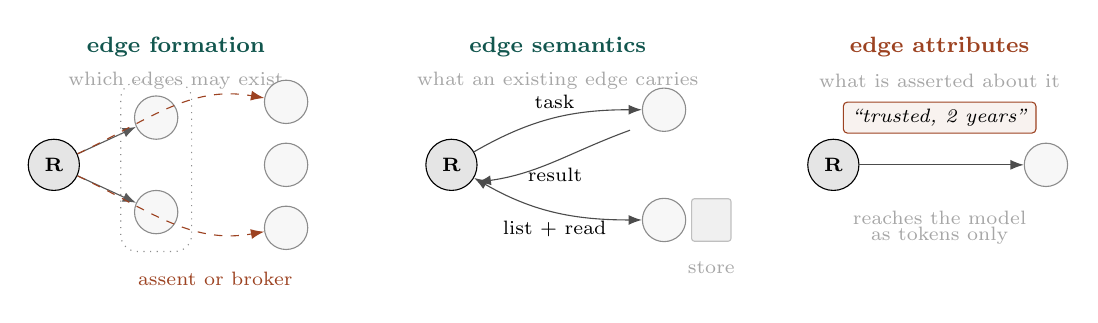
\begin{tikzpicture}[font=\small,>=Latex,
  ag/.style={circle,draw=black!45,fill=black!3,minimum size=5.5mm,inner sep=0pt},
  req/.style={circle,draw=black,fill=black!10,minimum size=6.5mm,inner sep=0pt,font=\scriptsize\bfseries},
  ttl/.style={font=\footnotesize\bfseries,align=center}]

% ---- panel 1: formation
\begin{scope}
  \node[ttl,arch] at (1.55,2.05) {edge formation};
  \node[font=\scriptsize,gray!70,align=center] at (1.55,1.62) {which edges may exist};
  \node[req] (R1) at (0,0.55) {R};
  \node[ag] (a1) at (1.3,1.15) {}; \node[ag] (a2) at (1.3,-0.05) {};
  \draw[->,black!65] (R1) -- (a1); \draw[->,black!65] (R1) -- (a2);
  \draw[dotted,black!45,rounded corners=6pt] (0.85,-0.55) rectangle (1.75,1.6);
  \node[ag] (b1) at (2.95,1.35) {}; \node[ag] (b2) at (2.95,0.55) {}; \node[ag] (b3) at (2.95,-0.25) {};
  \draw[->,dashed,attr] (R1) to[out=25,in=170] (b1);
  \draw[->,dashed,attr] (R1) to[out=-25,in=190] (b3);
  \node[font=\scriptsize,attr] at (2.05,-0.9) {assent or broker};
\end{scope}

% ---- panel 2: semantics
\begin{scope}[xshift=5.05cm]
  \node[ttl,arch] at (1.35,2.05) {edge semantics};
  \node[font=\scriptsize,gray!70,align=center] at (1.35,1.62) {what an existing edge carries};
  \node[req] (R2) at (0,0.55) {R};
  \node[ag] (c1) at (2.7,1.25) {}; \node[ag] (c2) at (2.7,-0.15) {};
  \draw[->,black!70] (R2) to[out=30,in=180] node[midway,above,font=\scriptsize,black]{task} (c1);
  \draw[<-,black!70] ([yshift=-2.2mm]R2.east) to[out=8,in=200] node[midway,below,font=\scriptsize,black,yshift=1pt]{result} ([xshift=-1.5mm,yshift=-2.6mm]c1.west);
  \draw[<->,black!70] (R2) to[out=-30,in=180] node[midway,below,font=\scriptsize,black]{list + read} (c2);
  \draw[black!25,fill=black!6,rounded corners=1pt] (3.05,-0.42) rectangle (3.55,0.12);
  \node[font=\scriptsize,gray!70] at (3.3,-0.75) {store};
\end{scope}

% ---- panel 3: attributes
\begin{scope}[xshift=9.9cm]
  \node[ttl,attr] at (1.35,2.05) {edge attributes};
  \node[font=\scriptsize,gray!70,align=center] at (1.35,1.62) {what is asserted about it};
  \node[req] (R3) at (0,0.55) {R};
  \node[ag] (d1) at (2.7,0.55) {};
  \draw[->,black!70] (R3) -- (d1);
  \node[draw=attr,fill=attr!7,rounded corners=1.5pt,inner sep=2.5pt,font=\scriptsize,align=center]
    at (1.35,1.15) {\textit{``trusted, 2 years''}};
  \node[font=\scriptsize,gray!70,align=center] at (1.35,-0.25) {reaches the model\\[-2pt]as tokens only};
\end{scope}
\end{tikzpicture}
\caption{The three axes, drawn on $G=(V,E)$. \arch{Formation} and \arch{semantics} are
enforced: a coordination layer refuses an edge that may not form and a request an edge does
not carry. \txt{Attributes} are never checked by anything---they arrive in a prompt, which
is why asking whether a model acts on them is a real question rather than a tautology. Each
regime supplies a characteristic value on all three (Table~\ref{tab:axes}), and a study that
compares public with private moves all three at once.}
\label{fig:axes}
\end{figure}
\fi

Table~\ref{tab:axes} is what each corner supplies on each axis --- the bundles unpacked.

\begin{table}[t]
\centering\small
\caption{The three axes, and what each regime supplies on it. Formation and semantics
are enforced by a coordination layer on every call; attributes only ever reach a model
as text. A study that compares a public network to a private one moves all three.}
\label{tab:axes}
\begin{tabular}{@{}p{0.155\linewidth}p{0.375\linewidth}p{0.375\linewidth}@{}}
\toprule
& \textbf{Public} & \textbf{Private} \\
\midrule
\arch{Edge\newline formation}
& Unilateral. Anyone in the directory is addressable; matching is by declared
  relevance. \textbf{Lateral topology}: wide and shallow, many weak ties.
& Bilateral or brokered. A counterpart is reachable because of a prior tie or an
  introduction. \textbf{Longitudinal topology}: narrow and deep, few strong ties. \\
\addlinespace[2pt]
\arch{Edge\newline semantics}
& Sandboxed by default. A counterpart accepts a task and returns a result; its store
  stays opaque. Interaction is one-shot request/response.
& Openable. Shared workspaces, persistent namespaces, a store that may be listed and
  read---affordable precisely because the tie exists. \\
\addlinespace[2pt]
\txt{Edge\newline attributes}
& Platform-computed for strangers: reputation scores, ratings, usage counts,
  verification badges.
& Carried by the relationship: tenure, who introduced whom, how the last
  collaboration went, who is answerable. \\
\bottomrule
\end{tabular}
\end{table}

\ifcompact\else Figure~\ref{fig:axes} draws the three on the graph.\fi The rest of this
section takes them one at a time.

\ifcompact
\paragraph{The two topologies are the substance of the formation axis.} A public directory
buys \emph{breadth}: a rare requirement finds someone and---less obviously---a claim can be
put to a second source. A private roster buys \emph{depth}: fewer counterparts, each
already paid for, each with a history. These are not two settings of one dial; they are the
returns on two different edge prices. Which links form, and at what price, is strategic
network formation \citep{jackson1996}, and the agent setting differs in that the price is
conventionally zero. On \arch{semantics}, exposure follows the tie---one does not open a
working directory to a stranger---but the axis is separately settable, and a capability
kernel expresses both settings as grants over different namespaces, so a condition is a set
of capabilities rather than a different codebase \citep{a2a2025}. On \txt{attributes}, both
regimes carry a characteristic form of trust-conveying metadata that no runtime checks: a
public network computes a score about a stranger, a private one carries a history about an
acquaintance. Both rest on the same assumption---that an agent builds a representation of
its counterpart from what it is told and acts differently because of it.

\else
\paragraph{Edge formation} is which edges a requester may create: the scope of the
directory it can enumerate and address. This is the axis the word ``public'' usually
refers to, and the one broadcast networks for agents are built around---an agent
publishes what it needs and what it offers, and the network routes to whoever is
relevant \citep{eigenflux}. Which links form, and at what price, is strategic network
formation \citep{jackson1996}; the agent setting differs in that the price is
conventionally zero.

The two topologies are the substance of the axis. A public directory buys
\emph{breadth}: a rare requirement finds someone, and---less obviously---a claim can be
put to a second source. A private roster buys \emph{depth}: fewer counterparts, each
already paid for, each with a history. Breadth and depth are not two settings of one
dial; they are the returns on two different edge prices.

\paragraph{Edge semantics} is what an existing edge carries. A counterpart may accept a
task and return a result while revealing nothing else, or expose a store to be listed
and read. The distinction is not ours: it separates agent-to-agent task protocols, which
deliberately keep a counterpart opaque \citep{a2a2025}, from granted resource scopes, in
which one principal hands another read access to files. It maps onto the regimes because
exposure follows the tie---one does not open a working directory to a stranger---but it
is separately settable, and a capability kernel expresses both as grants over different
namespaces, so a condition is a set of capabilities rather than a different codebase.

\paragraph{Edge attributes} is what is asserted \emph{about} an edge. Both regimes have
a characteristic form of it, and both are trust-conveying metadata that no runtime
checks: a public network computes a score about a stranger, a private one carries a
history about an acquaintance. They rest on the same assumption---that an agent builds
a representation of its counterpart from what it is told, and acts differently because
of it.

\fi

\subsection{Why these three and not nine}

The literature on ties, teams and open innovation supplies at least nine relational
dimensions---membership openness, identity continuity, shared-state depth, repeated
interaction, relationship origin, prior trust, shared goals, accountability, exit cost.
They are not nine degrees of freedom: in a deployed system an open directory brings weak
identity, which brings diffuse accountability, which brings low exit cost. The three-way
grouping breaks that coupling the one way a controlled study can. Formation and semantics
are properties of the interaction layer---independently settable, checked on every call,
not open to argument by a model. Attributes are properties of the people behind the agents;
a harness cannot instantiate them, only \emph{assert} them. That asymmetry is the
experiment rather than a limitation to apologise for: deployed networks communicate trust,
alignment, attribution and tenure as text on cards, so asking whether a model acts on that
text asks whether a large part of agent-network design does anything at all.

\ifcompact
\subsection{Two corrections the framework has to carry}

Both fall out of taking the edge, rather than visibility, as the primitive. First,
\textbf{a public network's noise is partly a feature}: a requester who can address many
counterparts can put the same question to a second one, and contradiction is
\emph{detectable}, so a roster that filters misinformation out before it arrives also
removes the second source needed to catch what does arrive. Whether the filter or the
redundancy dominates is empirical, and the framework must not settle it by calling breadth
a cost. Second, \textbf{an endorsement is not an introduction}, and they sit on different
axes. \txt{``This counterpart is reliable''} is an attribute: text on an edge that already
exists. \arch{An introduction that makes a third agent addressable} is formation: it
changes the graph. A framework that files both under ``trust'' predicts that a private
network's advantage comes from what it knows about its members; the decomposition predicts
something narrower---that only the half which changes reachability can do work---and
\S\ref{sec:evidence} reports which way it went.
\else
\subsection{Two corrections the framework has to carry}

Both fall out of taking the edge, rather than visibility, as the primitive.

\paragraph{A public network's noise is partly a feature.} The usual complaint is that an
open directory is full of unvetted claims. It is---but a requester who can address many
counterparts can put the same question to a second one, and contradiction is
\emph{detectable}. A roster that filters misinformation out before it arrives also
removes the second source needed to catch what does arrive. Whether the filter or the
redundancy dominates is an empirical question, not a definitional one, and the framework
must not settle it by calling breadth a cost.

\paragraph{An endorsement is not an introduction.} These are on different axes and are
routinely conflated. \txt{``This counterpart is reliable''} is an attribute: text, on an
edge that already exists. \arch{An introduction that makes a third agent addressable} is
formation: it changes the graph. A framework that files both under ``trust'' predicts
that a private network's advantage comes from what it knows about its members. The
decomposition predicts something narrower---that only the half which changes reachability
can do work---and \S\ref{sec:evidence} reports which way it went.
\fi

\section{Making each axis measurable}
\label{sec:quantifying}

The framework is only useful if each axis can be set independently and each regime's
claimed advantage can be priced. This section states what that requires; the instrument
that implements it is Appendix~\ref{app:instrument}.

\paragraph{One system, three switches.} Model, runtime, task, answer key and
coordination kernel are held fixed. A condition is a set of capability grants, not a
different codebase, so \arch{formation} (which cards a requester may enumerate and
address), \arch{semantics} (whether a counterpart returns an answer or exposes a store)
and \txt{attributes} (what the cards say about themselves and each other) move one at a
time. Formation and semantics are refused by the kernel when violated; attributes reach
the model only as tokens, which is what makes the third axis a real test rather than a
tautology.

\paragraph{A task class where pooling is forced.} Each episode is a hidden-profile
deliverable: the facts a correct artifact needs are distributed across counterparts so
that no single agent, including the requester, holds enough \citep{stasser1985}. Two
parameters make the axes bite. \metric{E} is the share of required facts placed
\emph{outside} the roster, which is the dose on the formation axis---at $E=0$ a private
network needs nothing it cannot already reach, and the axis must show no effect.
Distractors plant contradicting values on counterparts other than the true holder, so
that a second source has something to catch.

\paragraph{Metrics with no judge on any primary number.} Every fact is a number, a date,
a name or an enum, and the deliverable is scored by exact match after a normalization
rule fixed before the keys were written. This yields requirement $F_1$ as the task
score. Around it sit four quantities that price what a score costs:

\begin{itemize}[leftmargin=1.4em,itemsep=1pt,topsep=2pt]
\item \metric{useful sources} --- counterparts contacted that held a needed fact. The
      mechanism variable for formation.
\item \metric{pollution absorbed} and \metric{invented} --- a distractor's value
      appearing in the artifact, split by whether the agent was ever shown it. The
      second is fabrication, and it is the failure mode of a starved requester.
\item \metric{tokens} and \metric{contacts} --- the price of the arm, and, since each
      contact discloses the goal, its exposure.
\end{itemize}

An axis is not evaluated by its effect on $F_1$ alone. \arch{Semantics}, for instance,
buys accuracy and is charged in tokens; reporting only the first half would make the
private regime look better than the exchange rate supports.

\paragraph{Delivery is reported before any contrast.} A trial that produced no artifact
is a missing observation, not a score of zero, and averaging it in as zero converts an
outage into an effect. We found this the expensive way: one sweep lost 27\% of its
trials to transport failures, the losses landed unevenly across cells, and the resulting
curve was legible as a scaling result until the delivery rates were tabulated
(Appendix~\ref{app:retracted}). Every contrast we report is therefore preceded by a
per-cell delivery table, is computed both conditional on delivery and with losses scored
as zero, and is treated as uninterpretable when delivery differs across compared cells
by more than 15 points.

\section{The combination problem}
\label{sec:combination}

Three axes with two settings each give eight configurations, and no deployed network is
a corner. A roster with an introduction protocol is public on formation for the agents
it can reach through a broker and private for everyone else; an enterprise workspace is
private on formation and fully open on semantics. The design question is not which
regime wins but \textbf{which configuration a given setting should hold}, and that
requires each axis to be priced separately---which is what \S\ref{sec:quantifying}
buys.

\paragraph{The axes are not equally live.} A configuration search is only interesting if
more than one dimension moves the outcome. Our measurements so far
(\S\ref{sec:evidence}) put the three weights at roughly $0.23$, $0.08$ and $0$ on
requirement $F_1$, which collapses the search: pick a point on formation and the other
two are free. We report that collapse rather than dressing it as an optimisation,
because it is the honest reading of one task family---and because it makes the next
question sharp.

\paragraph{Scenarios are the test of whether the weights are constants.} The collapse
above was measured on a single task class: facts held by different agents, aggregated
into one deliverable. That class is maximally favourable to formation---reach is
literally what it asks for---and maximally unfavourable to semantics, since there is no
shared artifact to co-edit. If the three weights are properties of the framework, they
should hold elsewhere. If they are properties of the task, they will move, and the
combination problem becomes real.

\begin{table}[t]
\centering\small
\caption{Three settings, and what each predicts for the weight on each axis. These are
predictions the framework makes and does not yet have evidence for; the task families
are specified in Appendix~\ref{app:scenarios}.}
\label{tab:scenarios}
\begin{tabular}{@{}p{0.20\linewidth}p{0.30\linewidth}p{0.13\linewidth}p{0.13\linewidth}p{0.13\linewidth}@{}}
\toprule
\textbf{Setting} & \textbf{What a task looks like} & \textbf{formation} & \textbf{semantics} & \textbf{attributes} \\
\midrule
Enterprise team & Co-edit one artifact; the people are known; the context is the
  bottleneck & low & \textbf{high} & low \\
\addlinespace[2pt]
Personal errand & Find the one counterpart who can do a specific thing; no
  relationship needed after & \textbf{high} & low & medium \\
\addlinespace[2pt]
Personal social & Reach a person through someone; the introduction is the product &
  \textbf{high, brokered} & low & \textbf{high} \\
\bottomrule
\end{tabular}
\end{table}

The enterprise row is the sharpest test, because it predicts the reverse of what we
measured: when everyone needed is already reachable, formation has no work left to do,
and the shared store that cost 11k tokens for a small gain in a pooling task should pay
for itself when the deliverable is edited jointly. A framework that only ever produces
``formation dominates'' is a restatement of the task; one that predicts where formation
stops dominating, and is then held to it, is a framework.

\paragraph{What an optimum means here.} An optimum is a configuration, not a size. On
formation it is a \emph{funnel depth}: how far past the roster a requester should be
allowed to reach---own roster, one brokered hop, two hops, open directory---given that
each additional layer widens reach and weakens recourse. The marginal return on a layer
is the number of \emph{independent} sources it adds, which saturates; the marginal cost
is what a claim from that layer is worth, which decays. The crossing is the depth. Stated
this way the optimum is measurable per scenario rather than argued per regime.

\ifcompact
\section{Evidence so far}
\label{sec:evidence}

We have run the decomposition on one task family: 582 episodes across sixteen sweeps, one
model family, one kernel. The full record---every result, the nulls, and one
retraction---is Appendix~\ref{app:experiments}.


\begin{figure}[t]
\centering
\definecolor{openarm}{HTML}{2A78D6}
\definecolor{bndarm}{HTML}{C4551F}
\begin{tikzpicture}[x=1.05cm,y=1.2cm,font=\small]
\draw[gray!22] (-0.2,0.552) -- (7.7,0.552);
\node[anchor=east,gray!70,font=\scriptsize] at (-0.32,0.552) {0.5};
\draw[gray!22] (-0.2,1.241) -- (7.7,1.241);
\node[anchor=east,gray!70,font=\scriptsize] at (-0.32,1.241) {0.6};
\draw[gray!22] (-0.2,1.931) -- (7.7,1.931);
\node[anchor=east,gray!70,font=\scriptsize] at (-0.32,1.931) {0.7};
\draw[gray!22] (-0.2,2.621) -- (7.7,2.621);
\node[anchor=east,gray!70,font=\scriptsize] at (-0.32,2.621) {0.8};
\draw[gray!22] (-0.2,3.310) -- (7.7,3.310);
\node[anchor=east,gray!70,font=\scriptsize] at (-0.32,3.310) {0.9};
\draw[gray!22] (-0.2,4.000) -- (7.7,4.000);
\node[anchor=east,gray!70,font=\scriptsize] at (-0.32,4.000) {1.0};
\draw[gray!55] (-0.2,0.000) -- (7.7,0.000);
\node[anchor=north,gray!70,font=\scriptsize] at (0.00,-0.080) {$0.0$};
\node[anchor=north,gray!70,font=\scriptsize] at (3.10,-0.080) {$0.3$};
\node[anchor=north,gray!70,font=\scriptsize] at (7.20,-0.080) {$0.7$};
\draw[openarm,line width=1.1pt] (0.00,2.779) -- (3.10,2.559) -- (7.20,2.641);
\draw[openarm!65,line width=.8pt] (0.00,2.345) -- (0.00,3.200);
\draw[openarm!65,line width=.8pt] (-0.08,2.345) -- (0.08,2.345);
\draw[openarm!65,line width=.8pt] (-0.08,3.200) -- (0.08,3.200);
\filldraw[openarm] (0.00,2.779) circle (2.3pt);
\draw[openarm!65,line width=.8pt] (3.10,2.076) -- (3.10,3.007);
\draw[openarm!65,line width=.8pt] (3.02,2.076) -- (3.18,2.076);
\draw[openarm!65,line width=.8pt] (3.02,3.007) -- (3.18,3.007);
\filldraw[openarm] (3.10,2.559) circle (2.3pt);
\draw[openarm!65,line width=.8pt] (7.20,2.386) -- (7.20,2.910);
\draw[openarm!65,line width=.8pt] (7.12,2.386) -- (7.28,2.386);
\draw[openarm!65,line width=.8pt] (7.12,2.910) -- (7.28,2.910);
\filldraw[openarm] (7.20,2.641) circle (2.3pt);
\draw[bndarm,line width=1.1pt] (0.00,2.545) -- (3.10,1.786) -- (7.20,0.717);
\draw[bndarm!65,line width=.8pt] (0.00,1.979) -- (0.00,3.076);
\draw[bndarm!65,line width=.8pt] (-0.08,1.979) -- (0.08,1.979);
\draw[bndarm!65,line width=.8pt] (-0.08,3.076) -- (0.08,3.076);
\filldraw[bndarm] (0.00,2.545) circle (2.3pt);
\draw[bndarm!65,line width=.8pt] (3.10,1.379) -- (3.10,2.200);
\draw[bndarm!65,line width=.8pt] (3.02,1.379) -- (3.18,1.379);
\draw[bndarm!65,line width=.8pt] (3.02,2.200) -- (3.18,2.200);
\filldraw[bndarm] (3.10,1.786) circle (2.3pt);
\draw[bndarm!65,line width=.8pt] (7.20,0.338) -- (7.20,1.124);
\draw[bndarm!65,line width=.8pt] (7.12,0.338) -- (7.28,0.338);
\draw[bndarm!65,line width=.8pt] (7.12,1.124) -- (7.28,1.124);
\filldraw[bndarm] (7.20,0.717) circle (2.3pt);
\node[openarm,anchor=south,font=\scriptsize\bfseries] at (5.3,2.941) {open};
\node[bndarm,anchor=north,font=\scriptsize\bfseries] at (5.4,0.377) {bounded};
\draw[black!50,line width=.7pt] (0.42,3.200) -- (0.62,3.200) -- (0.62,1.979) -- (0.42,1.979);
\draw[black!35,line width=.6pt] (0.62,2.593) -- (1.15,1.241);
\node[black!70,font=\scriptsize,align=left,anchor=west] at (1.18,1.241) {no gap at zero dose:\\[-2pt]$+0.034$, CI spans $0$};
\node[anchor=north,gray!70,font=\scriptsize] at (3.6,-0.480) {$E$ --- share of required facts placed outside the roster};
\end{tikzpicture}
\caption{The formation effect is reach, and the dose-response says so. \metric{E} is the
share of a task's required facts placed outside the roster; bars are 95\% percentile
bootstrap intervals over episodes. Four things hold at once, and the axis needs all four:
the contrast \textbf{vanishes at zero dose}, which is the control it had to pass; the arm
that cannot be affected is \textbf{flat} across all three doses; the mechanism variable
tracks the dose (the bounded arm's useful sources fall $4.36 \to 3.17 \to 1.26$); and
fabrication appears only as sources dry up ($0 \to 0.139 \to 0.333$ per task).}
\label{fig:dose}
\end{figure}


\begin{center}\small
\begin{tabular}{@{}p{0.28\linewidth}p{0.64\linewidth}@{}}
\toprule
\textbf{Finding} & \textbf{Evidence} \\
\midrule
Only formation is an intervention
& The two diagonals of one factorial give $0.181$ and $0.314$ on the same episodes; the
  factorial recovers $0.248$ formation and $0.066$ semantics (CI $[+0.012,+0.119]$, $+19$k
  tokens), and $\approx\!0$ attributes. 56 contrasts per beat against a chance floor of
  $2.8$; the two that cleared reverse sign between beats of the same episodes; a
  length-matched placebo of two neutral lines moves the score $+0.005$. \\
\addlinespace[2pt]
The formation effect is reach
& Dose-response in \metric{E} (Figure~\ref{fig:dose}): $+0.034$ (CI $[-0.067,+0.137]$) at
  $E=0$, $+0.111$ at $0.3$, $+0.279$ at $0.7$. The public arm is flat across all three
  doses; the private arm's useful sources fall $4.36 \to 3.17 \to 1.26$. \\
\addlinespace[2pt]
A roster sees less bad information and believes more of it
& Shown a third as much planted misinformation; writes $0.269$ against $0.094$ instances
  per task into the deliverable ($+0.175$, CI $[+0.105,+0.242]$). Across 287 and 286
  delivered tasks the public arms fabricated once, the private arms 58 times. Matching on
  sources obtained does not close it (2.4\% against 18.1\% at four sources). \\
\addlinespace[2pt]
An introduction does work an endorsement does not
& One brokered hop recovers $+0.140$ (CI $[+0.073,+0.204]$) of a $0.304$ gap, replicating
  within three edge-cost strata, and cuts fabrication $0.223 \to 0.057$. Read-all with deep
  ties only inside the roster is indistinguishable from full openness ($+0.019$). Both are
  formation manipulations; every attribute manipulation is flat. \\
\addlinespace[2pt]
\textbf{The bounded arm is weakly dominated}
& It never scores higher, and it spends $\sim$19k more tokens per task at every $E$
  including $E=0$, where its roster holds everything the task needs and it ties on accuracy.
  Its one better column---1.7 fewer counterparts disclosed to---appears only at $E=0.7$,
  where it also scores $0.279$ lower and fabricates in a third of its tasks. \\
\bottomrule
\end{tabular}
\end{center}

\paragraph{So if a private agent network is worth building, our measurements do not contain
the reason.} Three candidates sit outside the scorer. \emph{Confidentiality}: our only proxy
is how many counterparts learn the goal, and it favours the bounded arm only where that arm
has failed. \emph{Recourse}: accountability needs a second encounter, and every episode here
is a cold start (\S\ref{sec:lifecycle}). \emph{Adversaries}: 36 of 100 cards carry plausible
tags and no knowledge, but every agent that is asked answers honestly. What the data does
rule out is the justification most often given---that a bounded network produces better
information. It produces worse information, more expensively. Two limits are ours rather
than the framework's: one model family carries every sweep with a live main effect, and the
scenario predictions of \S\ref{sec:combination} are predictions.
\else
\section{Evidence so far}
\label{sec:evidence}

We have run the decomposition on one task family: 582 episodes across sixteen sweeps, one
model family, one kernel. The full inventory, every result including the nulls and one
retraction, is Appendix~\ref{app:experiments}. Five findings bear on the framework.

\paragraph{Only formation is an intervention.} A naive public-versus-private contrast
returns $0.181$ or $0.314$ on requirement $F_1$ depending on which pairing is called public
and which private---the two diagonals of one factorial, on one set of episodes. The
factorial recovers what neither diagonal isolates: $0.248$ (CI $[+0.194, +0.302]$) from edge
formation, $0.066$ (CI $[+0.012, +0.119]$, and 19k tokens a task) from edge semantics, and
nothing distinguishable from zero on attributes. That axis was tested across 56 contrasts
per beat against a chance floor of $2.8$; two cleared and reversed sign between beats of the
same episodes, and a length-matched placebo of two neutral lines moved the score by
$+0.005$. Prior trust and attribution, the two properties deployed reputation systems carry,
are the flattest measurements in the set.


\begin{figure}[t]
\centering
\definecolor{openarm}{HTML}{2A78D6}
\definecolor{bndarm}{HTML}{C4551F}
\begin{tikzpicture}[x=1.05cm,y=1.2cm,font=\small]
\draw[gray!22] (-0.2,0.552) -- (7.7,0.552);
\node[anchor=east,gray!70,font=\scriptsize] at (-0.32,0.552) {0.5};
\draw[gray!22] (-0.2,1.241) -- (7.7,1.241);
\node[anchor=east,gray!70,font=\scriptsize] at (-0.32,1.241) {0.6};
\draw[gray!22] (-0.2,1.931) -- (7.7,1.931);
\node[anchor=east,gray!70,font=\scriptsize] at (-0.32,1.931) {0.7};
\draw[gray!22] (-0.2,2.621) -- (7.7,2.621);
\node[anchor=east,gray!70,font=\scriptsize] at (-0.32,2.621) {0.8};
\draw[gray!22] (-0.2,3.310) -- (7.7,3.310);
\node[anchor=east,gray!70,font=\scriptsize] at (-0.32,3.310) {0.9};
\draw[gray!22] (-0.2,4.000) -- (7.7,4.000);
\node[anchor=east,gray!70,font=\scriptsize] at (-0.32,4.000) {1.0};
\draw[gray!55] (-0.2,0.000) -- (7.7,0.000);
\node[anchor=north,gray!70,font=\scriptsize] at (0.00,-0.080) {$0.0$};
\node[anchor=north,gray!70,font=\scriptsize] at (3.10,-0.080) {$0.3$};
\node[anchor=north,gray!70,font=\scriptsize] at (7.20,-0.080) {$0.7$};
\draw[openarm,line width=1.1pt] (0.00,2.779) -- (3.10,2.559) -- (7.20,2.641);
\draw[openarm!65,line width=.8pt] (0.00,2.345) -- (0.00,3.200);
\draw[openarm!65,line width=.8pt] (-0.08,2.345) -- (0.08,2.345);
\draw[openarm!65,line width=.8pt] (-0.08,3.200) -- (0.08,3.200);
\filldraw[openarm] (0.00,2.779) circle (2.3pt);
\draw[openarm!65,line width=.8pt] (3.10,2.076) -- (3.10,3.007);
\draw[openarm!65,line width=.8pt] (3.02,2.076) -- (3.18,2.076);
\draw[openarm!65,line width=.8pt] (3.02,3.007) -- (3.18,3.007);
\filldraw[openarm] (3.10,2.559) circle (2.3pt);
\draw[openarm!65,line width=.8pt] (7.20,2.386) -- (7.20,2.910);
\draw[openarm!65,line width=.8pt] (7.12,2.386) -- (7.28,2.386);
\draw[openarm!65,line width=.8pt] (7.12,2.910) -- (7.28,2.910);
\filldraw[openarm] (7.20,2.641) circle (2.3pt);
\draw[bndarm,line width=1.1pt] (0.00,2.545) -- (3.10,1.786) -- (7.20,0.717);
\draw[bndarm!65,line width=.8pt] (0.00,1.979) -- (0.00,3.076);
\draw[bndarm!65,line width=.8pt] (-0.08,1.979) -- (0.08,1.979);
\draw[bndarm!65,line width=.8pt] (-0.08,3.076) -- (0.08,3.076);
\filldraw[bndarm] (0.00,2.545) circle (2.3pt);
\draw[bndarm!65,line width=.8pt] (3.10,1.379) -- (3.10,2.200);
\draw[bndarm!65,line width=.8pt] (3.02,1.379) -- (3.18,1.379);
\draw[bndarm!65,line width=.8pt] (3.02,2.200) -- (3.18,2.200);
\filldraw[bndarm] (3.10,1.786) circle (2.3pt);
\draw[bndarm!65,line width=.8pt] (7.20,0.338) -- (7.20,1.124);
\draw[bndarm!65,line width=.8pt] (7.12,0.338) -- (7.28,0.338);
\draw[bndarm!65,line width=.8pt] (7.12,1.124) -- (7.28,1.124);
\filldraw[bndarm] (7.20,0.717) circle (2.3pt);
\node[openarm,anchor=south,font=\scriptsize\bfseries] at (5.3,2.941) {open};
\node[bndarm,anchor=north,font=\scriptsize\bfseries] at (5.4,0.377) {bounded};
\draw[black!50,line width=.7pt] (0.42,3.200) -- (0.62,3.200) -- (0.62,1.979) -- (0.42,1.979);
\draw[black!35,line width=.6pt] (0.62,2.593) -- (1.15,1.241);
\node[black!70,font=\scriptsize,align=left,anchor=west] at (1.18,1.241) {no gap at zero dose:\\[-2pt]$+0.034$, CI spans $0$};
\node[anchor=north,gray!70,font=\scriptsize] at (3.6,-0.480) {$E$ --- share of required facts placed outside the roster};
\end{tikzpicture}
\caption{The formation effect is reach, and the dose-response says so. \metric{E} is the
share of a task's required facts placed outside the roster; bars are 95\% percentile
bootstrap intervals over episodes. Four things hold at once, and the axis needs all four:
the contrast \textbf{vanishes at zero dose}, which is the control it had to pass; the arm
that cannot be affected is \textbf{flat} across all three doses; the mechanism variable
tracks the dose (the bounded arm's useful sources fall $4.36 \to 3.17 \to 1.26$); and
fabrication appears only as sources dry up ($0 \to 0.139 \to 0.333$ per task).}
\label{fig:dose}
\end{figure}


\paragraph{The formation effect is reach, and the dose-response says so.} With
\metric{E}---the share of required facts outside the roster---as the dose, the contrast runs
$+0.034$ (95\% CI $[-0.067, +0.137]$, spans zero) at $E=0$ (Figure~\ref{fig:dose}), $+0.111$
at $E = 0.3$ and $+0.279$ at $E = 0.7$. The zero-dose cell is the control the axis had to
pass and did: a private network that can already reach what a task needs is not worse. The
public arm is flat across all three doses ($0.823 / 0.791 / 0.803$), so the manipulation is
specific to the arm it should affect, and the mechanism variable tracks it---the private
arm's useful sources fall $4.36 \to 3.17 \to 1.26$.

\paragraph{A roster sees less bad information and believes more of it.} This is the one
result we did not design (Figure~\ref{fig:credulity}, in the appendix). The private arm is shown roughly a
quarter as much planted misinformation as the public arm, and writes it into the deliverable
\emph{more}---$0.269$ against $0.094$ instances per task (difference $+0.175$, CI
$[+0.105, +0.242]$). When it reaches no one at all it does not decline to answer: across
matched sets of 287 and 286 delivered tasks, the public arms fabricated a value once and the
private arms 58 times. Filtering misinformation out before it arrives also removes the
second source that would have caught it, which is the redundancy argument of
\S\ref{sec:framework} appearing as a failure mode rather than as a benefit. That explanation
is not the whole mechanism, and we say so because the tidier version is available and wrong:
among beats that obtained four useful sources the absorption rate is 2.4\% open against
18.1\% bounded, so starvation amplifies credulity without being all of it.

\ifcompact\else
\begin{figure}[t]
\centering
\definecolor{openarm}{HTML}{2A78D6}
\definecolor{bndarm}{HTML}{C4551F}
\definecolor{brokerc}{HTML}{9A7A3E}
\begin{tikzpicture}[x=1.05cm,y=1.05cm,font=\small]
\draw[gray!22] (0.645,-0.30) -- (0.645,3.45);
\node[gray!70,font=\scriptsize,anchor=north] at (0.645,-0.34) {0.5};
\draw[gray!22] (2.259,-0.30) -- (2.259,3.45);
\node[gray!70,font=\scriptsize,anchor=north] at (2.259,-0.34) {0.6};
\draw[gray!22] (3.873,-0.30) -- (3.873,3.45);
\node[gray!70,font=\scriptsize,anchor=north] at (3.873,-0.34) {0.7};
\draw[gray!22] (5.486,-0.30) -- (5.486,3.45);
\node[gray!70,font=\scriptsize,anchor=north] at (5.486,-0.34) {0.8};
\draw[gray!22] (7.100,-0.30) -- (7.100,3.45);
\node[gray!70,font=\scriptsize,anchor=north] at (7.100,-0.34) {0.9};
\draw[gray!30,line width=.5pt] (0,3.10) -- (7.25,3.10);
\draw[bndarm,line width=1.4pt] (0.807,3.10) -- (2.227,3.10);
\draw[bndarm,line width=1.4pt] (0.807,2.99) -- (0.807,3.21);
\draw[bndarm,line width=1.4pt] (2.227,2.99) -- (2.227,3.21);
\filldraw[bndarm] (1.501,3.10) circle (3.1pt);
\node[font=\scriptsize,anchor=west] at (2.387,3.10) {0.553};
\node[font=\scriptsize\bfseries,anchor=east,align=right] at (-0.22,3.21) {bounded, island};
\node[font=\scriptsize,gray!70,anchor=east,align=right] at (-0.22,2.93) {only its own roster};
\draw[gray!30,line width=.5pt] (0,2.26) -- (7.25,2.26);
\draw[brokerc,line width=1.4pt] (2.985,2.26) -- (4.534,2.26);
\draw[brokerc,line width=1.4pt] (2.985,2.15) -- (2.985,2.37);
\draw[brokerc,line width=1.4pt] (4.534,2.15) -- (4.534,2.37);
\filldraw[brokerc] (3.760,2.26) circle (3.1pt);
\node[font=\scriptsize,anchor=west] at (4.694,2.26) {0.693};
\node[font=\scriptsize\bfseries,anchor=east,align=right] at (-0.22,2.37) {bounded, one brokered hop};
\node[font=\scriptsize,gray!70,anchor=east,align=right] at (-0.22,2.09) {a roster member forwards};
\draw[gray!30,line width=.5pt] (0,1.42) -- (7.25,1.42);
\draw[openarm!62,line width=1.4pt] (5.164,1.42) -- (6.906,1.42);
\draw[openarm!62,line width=1.4pt] (5.164,1.31) -- (5.164,1.53);
\draw[openarm!62,line width=1.4pt] (6.906,1.31) -- (6.906,1.53);
\filldraw[openarm!62] (6.067,1.42) circle (3.1pt);
\node[font=\scriptsize,anchor=west] at (7.066,1.42) {0.836};
\node[font=\scriptsize\bfseries,anchor=east,align=right] at (-0.22,1.53) {read-all, deep only inside};
\node[font=\scriptsize,gray!70,anchor=east,align=right] at (-0.22,1.25) {sees everyone, knows twenty};
\draw[gray!30,line width=.5pt] (0,0.58) -- (7.25,0.58);
\draw[openarm,line width=1.4pt] (5.987,0.58) -- (6.826,0.58);
\draw[openarm,line width=1.4pt] (5.987,0.47) -- (5.987,0.69);
\draw[openarm,line width=1.4pt] (6.826,0.47) -- (6.826,0.69);
\filldraw[openarm] (6.406,0.58) circle (3.1pt);
\node[font=\scriptsize,anchor=west] at (6.986,0.58) {0.857};
\node[font=\scriptsize\bfseries,anchor=east,align=right] at (-0.22,0.69) {open};
\node[font=\scriptsize,gray!70,anchor=east,align=right] at (-0.22,0.41) {addresses anyone};
\node[gray!70,font=\scriptsize,anchor=north] at (3.550,-0.72) {requirement $F_1$ (95\% CI)};
\end{tikzpicture}
\caption{An introduction does work an endorsement does not. All four rows are formation
manipulations, and every one of them moves; every \txt{attribute} manipulation---including
the ones asserting exactly the trust a broker would carry---is flat. One brokered hop
recovers $+0.140$ (CI $[+0.073, +0.204]$) of the $0.304$ gap and cuts fabrication from
$0.223$ to $0.057$ per task; letting a bounded arm read the whole directory while keeping
deep relationships inside the roster is indistinguishable from full openness ($+0.019$,
spans zero). Depth of relationship is not what is bought here---a second reachable source
is.}
\label{fig:ladder}
\end{figure}
\fi

\paragraph{An introduction does work an endorsement does not.} A bounded roster given a
single brokered hop---one roster member may forward a request to a counterpart the requester
cannot address---recovers close to half the gap to the open arm, and most of the fabrication
with it; letting a bounded arm \emph{read} the whole directory while keeping deep
relationships inside the roster is indistinguishable from full openness
(Figure~\ref{fig:ladder}). Both are formation manipulations, and both move. Every attribute
manipulation is flat, including the ones asserting exactly the trust an introduction would
carry. This is the endorsement/introduction distinction of \S\ref{sec:framework} landing
where the framework said it would: what changes the graph does work, what describes it does
not.

\paragraph{On everything we measured, the bounded arm is weakly dominated.} The
decomposition invites a symmetric reading that the data does not support, so this is worth
stating without hedging.

\begin{center}\small
\begin{tabular}{@{}lrrr@{}}
\toprule
\textbf{bounded $-$ open} & \textbf{$E=0$} & \textbf{$E=0.3$} & \textbf{$E=0.7$} \\
\midrule
requirement $F_1$         & tie              & $-0.111^\ast$      & $-0.279^\ast$ \\
tokens per task           & $+18.8$k$^\ast$  & $+19.5$k$^\ast$    & $+19.1$k$^\ast$ \\
wall clock                & tie              & $+0.8$\,min$^\ast$ & $+0.5$\,min$^\ast$ \\
fabrications per task     & tie (both $0$)   & $+0.139^\ast$      & $+0.319^\ast$ \\
counterparts disclosed to & tie              & tie                & $-1.7^\ast$ \\
\bottomrule
\end{tabular}\\[1pt]
{\footnotesize $^\ast$ 95\% CI excludes zero.}
\end{center}

\noindent The $E=0$ column is the private network's best case: its roster already holds
every fact the task needs. It does not win there. It ties on accuracy and spends 38\% more
tokens to do it---an overhead of $+17.9$k in one harness generation and $+19.3$k in the
other, so not an artifact of either. Its growth is explained (the bounded arm searches its
twenty-card roster $6.8 \to 10.1 \to 16.2$ times as $E$ rises while its useful sources fall,
which is what looking harder for something that is not there costs); the baseline at $E=0$
is not. The one column where it looks better is disclosure, and only at $E=0.7$, where it
also scores $0.279$ lower and fabricates in a third of its tasks. \textbf{A network that
leaks less because it reached nobody has not protected anything.}

\paragraph{So if a private agent network is worth building, our measurements do not contain
the reason.} Three candidates sit outside the scorer, and each names its own experiment.
\emph{Confidentiality}: our only proxy is how many counterparts learn the goal, and it
favours the bounded arm only where that arm has failed---a real test needs a disclosure term
in the objective, not a by-product of contact count. \emph{Recourse}: accountability needs a
second encounter to mean anything, and every episode here is a cold start
(\S\ref{sec:lifecycle}). \emph{Adversaries}: 36 of 100 cards carry plausible tags and no
knowledge, but every agent that is asked answers honestly, so the defence a private network
exists to provide has nothing to defend against here. What the data does rule out is the
justification most often given: that a bounded network produces better information. It
produces worse information, more expensively.

Two further limits are ours rather than the framework's. One model family carries every
sweep with a live main effect---the second-model replication was run only at $E=0$, the
control cell, so model-independence is not established. And the scenario predictions of
\S\ref{sec:combination} are predictions.
\fi

\section{Further question: the two regimes scale on different bottlenecks}
\label{sec:scaling}

The framework invites a scaling question it does not answer, and unpacking the bundle
changes what the question is. The two corners do not grow along the same variable, so they
cannot degrade for the same reason.

A public network grows in $N$, the number of addressable counterparts, and $N$ is not
chosen by anyone. Coverage rises with it; so do search cost, verification cost and
exposure to counterparts nobody vetted. Its binding constraint is whether ranking can still
surface the right counterpart out of $N$.

A private network cannot grow in $N$: a roster is bounded by construction. It grows in
$d$, the number of brokered hops a request may travel, because that is the only way trusted
coverage increases. Its costs are not retrieval costs---they are the cost of asking a
broker to spend its own standing, and the decay of whatever recourse survives a chain of
introductions. Its binding constraint is path length and trust transitivity.

\begin{quote}
\textbf{Public networks scale through ranking; private networks scale through
relationships.} The open question the framework poses is not which is better at scale but
which degrades faster, under what task distribution, and whether a hybrid inherits the
better bottleneck from each.
\end{quote}

We can speak to the first of the two and not the second.

Within the range we can run, directory size does nothing. Growing the directory from 50
to 800 cards---16$\times$, with the roster held at twenty---leaves the open arm's score
flat ($0.800 \to 0.826$, CI spans zero) while search precision falls by roughly half and
tokens double. The arm pays for the extra difficulty rather than failing at it. We report
this null with a caveat earned the hard way: our first reading of this sweep was a
scaling result, and it was an outage (Appendix~\ref{app:retracted}).


\begin{figure}[t]
\centering
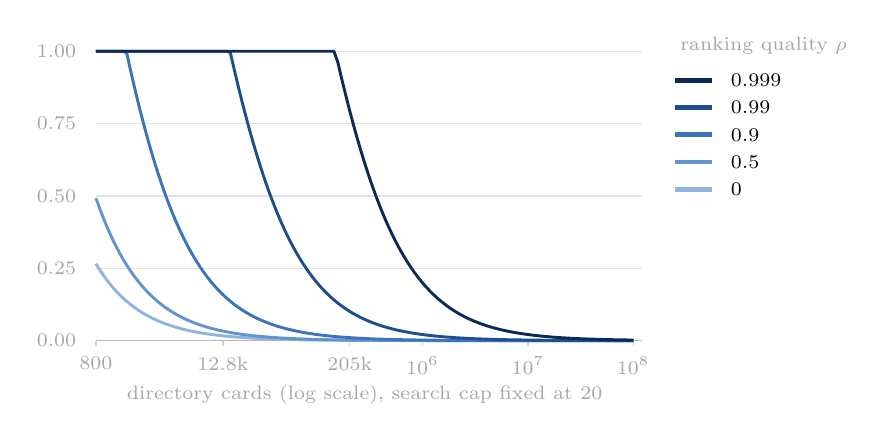
\begin{tikzpicture}[x=1.05cm,y=1.05cm,font=\small]
\draw[gray!22] (0,0.000) -- (6.60,0.000);
\node[gray!70,font=\scriptsize,anchor=east] at (-0.12,0.000) {0.00};
\draw[gray!22] (0,0.875) -- (6.60,0.875);
\node[gray!70,font=\scriptsize,anchor=east] at (-0.12,0.875) {0.25};
\draw[gray!22] (0,1.750) -- (6.60,1.750);
\node[gray!70,font=\scriptsize,anchor=east] at (-0.12,1.750) {0.50};
\draw[gray!22] (0,2.625) -- (6.60,2.625);
\node[gray!70,font=\scriptsize,anchor=east] at (-0.12,2.625) {0.75};
\draw[gray!22] (0,3.500) -- (6.60,3.500);
\node[gray!70,font=\scriptsize,anchor=east] at (-0.12,3.500) {1.00};
\draw[gray!55] (0,0) -- (6.60,0);
\draw[gray!35] (0.000,0) -- (0.000,-0.07);
\node[gray!70,font=\scriptsize,anchor=north] at (0.000,-0.08) {800};
\draw[gray!35] (1.536,0) -- (1.536,-0.07);
\node[gray!70,font=\scriptsize,anchor=north] at (1.536,-0.08) {12.8k};
\draw[gray!35] (3.071,0) -- (3.071,-0.07);
\node[gray!70,font=\scriptsize,anchor=north] at (3.071,-0.08) {205k};
\draw[gray!35] (3.949,0) -- (3.949,-0.07);
\node[gray!70,font=\scriptsize,anchor=north] at (3.949,-0.08) {$10^6$};
\draw[gray!35] (5.225,0) -- (5.225,-0.07);
\node[gray!70,font=\scriptsize,anchor=north] at (5.225,-0.08) {$10^7$};
\draw[gray!35] (6.500,0) -- (6.500,-0.07);
\node[gray!70,font=\scriptsize,anchor=north] at (6.500,-0.08) {$10^8$};
\definecolor{rc0}{HTML}{8FB4DE}
\definecolor{rc0p5}{HTML}{6394CE}
\definecolor{rc0p9}{HTML}{3B74BC}
\definecolor{rc0p99}{HTML}{1E4E8C}
\definecolor{rc0p999}{HTML}{0C2B54}
\draw[rc0,line width=1.05pt,line join=round] (0.0000,0.9309) -- (0.0464,0.8560) -- (0.0929,0.7872) -- (0.1393,0.7239) -- (0.1857,0.6657) -- (0.2321,0.6121) -- (0.2786,0.5629) -- (0.3250,0.5176) -- (0.3714,0.4760) -- (0.4179,0.4377) -- (0.4643,0.4025) -- (0.5107,0.3702) -- (0.5571,0.3404) -- (0.6036,0.3130) -- (0.6500,0.2879) -- (0.6964,0.2647) -- (0.7429,0.2434) -- (0.7893,0.2239) -- (0.8357,0.2059) -- (0.8821,0.1893) -- (0.9286,0.1741) -- (0.9750,0.1601) -- (1.0214,0.1472) -- (1.0679,0.1354) -- (1.1143,0.1245) -- (1.1607,0.1145) -- (1.2071,0.1053) -- (1.2536,0.0968) -- (1.3000,0.0890) -- (1.3464,0.0819) -- (1.3929,0.0753) -- (1.4393,0.0692) -- (1.4857,0.0637) -- (1.5321,0.0585) -- (1.5786,0.0538) -- (1.6250,0.0495) -- (1.6714,0.0455) -- (1.7179,0.0419) -- (1.7643,0.0385) -- (1.8107,0.0354) -- (1.8571,0.0326) -- (1.9036,0.0299) -- (1.9500,0.0275) -- (1.9964,0.0253) -- (2.0429,0.0233) -- (2.0893,0.0214) -- (2.1357,0.0197) -- (2.1821,0.0181) -- (2.2286,0.0166) -- (2.2750,0.0153) -- (2.3214,0.0141) -- (2.3679,0.0129) -- (2.4143,0.0119) -- (2.4607,0.0109) -- (2.5071,0.0101) -- (2.5536,0.0093) -- (2.6000,0.0085) -- (2.6464,0.0078) -- (2.6929,0.0072) -- (2.7393,0.0066) -- (2.7857,0.0061) -- (2.8321,0.0056) -- (2.8786,0.0051) -- (2.9250,0.0047) -- (2.9714,0.0044) -- (3.0179,0.0040) -- (3.0643,0.0037) -- (3.1107,0.0034) -- (3.1571,0.0031) -- (3.2036,0.0029) -- (3.2500,0.0026) -- (3.2964,0.0024) -- (3.3429,0.0022) -- (3.3893,0.0020) -- (3.4357,0.0019) -- (3.4821,0.0017) -- (3.5286,0.0016) -- (3.5750,0.0015) -- (3.6214,0.0013) -- (3.6679,0.0012) -- (3.7143,0.0011) -- (3.7607,0.0010) -- (3.8071,0.0010) -- (3.8536,0.0009) -- (3.9000,0.0008) -- (3.9464,0.0007) -- (3.9929,0.0007) -- (4.0393,0.0006) -- (4.0857,0.0006) -- (4.1321,0.0005) -- (4.1786,0.0005) -- (4.2250,0.0005) -- (4.2714,0.0004) -- (4.3179,0.0004) -- (4.3643,0.0004) -- (4.4107,0.0003) -- (4.4571,0.0003) -- (4.5036,0.0003) -- (4.5500,0.0003) -- (4.5964,0.0002) -- (4.6429,0.0002) -- (4.6893,0.0002) -- (4.7357,0.0002) -- (4.7821,0.0002) -- (4.8286,0.0002) -- (4.8750,0.0001) -- (4.9214,0.0001) -- (4.9679,0.0001) -- (5.0143,0.0001) -- (5.0607,0.0001) -- (5.1071,0.0001) -- (5.1536,0.0001) -- (5.2000,0.0001) -- (5.2464,0.0001) -- (5.2929,0.0001) -- (5.3393,0.0001) -- (5.3857,0.0001) -- (5.4321,0.0001) -- (5.4786,0.0000) -- (5.5250,0.0000) -- (5.5714,0.0000) -- (5.6179,0.0000) -- (5.6643,0.0000) -- (5.7107,0.0000) -- (5.7571,0.0000) -- (5.8036,0.0000) -- (5.8500,0.0000) -- (5.8964,0.0000) -- (5.9429,0.0000) -- (5.9893,0.0000) -- (6.0357,0.0000) -- (6.0821,0.0000) -- (6.1286,0.0000) -- (6.1750,0.0000) -- (6.2214,0.0000) -- (6.2679,0.0000) -- (6.3143,0.0000) -- (6.3607,0.0000) -- (6.4071,0.0000) -- (6.4536,0.0000) -- (6.5000,0.0000);
\draw[rc0p5,line width=1.05pt,line join=round] (0.0000,1.7241) -- (0.0464,1.5950) -- (0.0929,1.4748) -- (0.1393,1.3632) -- (0.1857,1.2595) -- (0.2321,1.1632) -- (0.2786,1.0740) -- (0.3250,0.9913) -- (0.3714,0.9147) -- (0.4179,0.8438) -- (0.4643,0.7782) -- (0.5107,0.7176) -- (0.5571,0.6615) -- (0.6036,0.6097) -- (0.6500,0.5619) -- (0.6964,0.5177) -- (0.7429,0.4769) -- (0.7893,0.4393) -- (0.8357,0.4046) -- (0.8821,0.3726) -- (0.9286,0.3430) -- (0.9750,0.3158) -- (1.0214,0.2908) -- (1.0679,0.2676) -- (1.1143,0.2463) -- (1.1607,0.2267) -- (1.2071,0.2087) -- (1.2536,0.1920) -- (1.3000,0.1767) -- (1.3464,0.1626) -- (1.3929,0.1496) -- (1.4393,0.1376) -- (1.4857,0.1266) -- (1.5321,0.1165) -- (1.5786,0.1072) -- (1.6250,0.0986) -- (1.6714,0.0907) -- (1.7179,0.0834) -- (1.7643,0.0767) -- (1.8107,0.0706) -- (1.8571,0.0649) -- (1.9036,0.0597) -- (1.9500,0.0549) -- (1.9964,0.0505) -- (2.0429,0.0465) -- (2.0893,0.0427) -- (2.1357,0.0393) -- (2.1821,0.0362) -- (2.2286,0.0332) -- (2.2750,0.0306) -- (2.3214,0.0281) -- (2.3679,0.0259) -- (2.4143,0.0238) -- (2.4607,0.0219) -- (2.5071,0.0201) -- (2.5536,0.0185) -- (2.6000,0.0170) -- (2.6464,0.0156) -- (2.6929,0.0144) -- (2.7393,0.0132) -- (2.7857,0.0122) -- (2.8321,0.0112) -- (2.8786,0.0103) -- (2.9250,0.0095) -- (2.9714,0.0087) -- (3.0179,0.0080) -- (3.0643,0.0074) -- (3.1107,0.0068) -- (3.1571,0.0062) -- (3.2036,0.0057) -- (3.2500,0.0053) -- (3.2964,0.0048) -- (3.3429,0.0045) -- (3.3893,0.0041) -- (3.4357,0.0038) -- (3.4821,0.0035) -- (3.5286,0.0032) -- (3.5750,0.0029) -- (3.6214,0.0027) -- (3.6679,0.0025) -- (3.7143,0.0023) -- (3.7607,0.0021) -- (3.8071,0.0019) -- (3.8536,0.0018) -- (3.9000,0.0016) -- (3.9464,0.0015) -- (3.9929,0.0014) -- (4.0393,0.0013) -- (4.0857,0.0012) -- (4.1321,0.0011) -- (4.1786,0.0010) -- (4.2250,0.0009) -- (4.2714,0.0008) -- (4.3179,0.0008) -- (4.3643,0.0007) -- (4.4107,0.0006) -- (4.4571,0.0006) -- (4.5036,0.0005) -- (4.5500,0.0005) -- (4.5964,0.0005) -- (4.6429,0.0004) -- (4.6893,0.0004) -- (4.7357,0.0004) -- (4.7821,0.0003) -- (4.8286,0.0003) -- (4.8750,0.0003) -- (4.9214,0.0003) -- (4.9679,0.0002) -- (5.0143,0.0002) -- (5.0607,0.0002) -- (5.1071,0.0002) -- (5.1536,0.0002) -- (5.2000,0.0002) -- (5.2464,0.0001) -- (5.2929,0.0001) -- (5.3393,0.0001) -- (5.3857,0.0001) -- (5.4321,0.0001) -- (5.4786,0.0001) -- (5.5250,0.0001) -- (5.5714,0.0001) -- (5.6179,0.0001) -- (5.6643,0.0001) -- (5.7107,0.0001) -- (5.7571,0.0001) -- (5.8036,0.0001) -- (5.8500,0.0000) -- (5.8964,0.0000) -- (5.9429,0.0000) -- (5.9893,0.0000) -- (6.0357,0.0000) -- (6.0821,0.0000) -- (6.1286,0.0000) -- (6.1750,0.0000) -- (6.2214,0.0000) -- (6.2679,0.0000) -- (6.3143,0.0000) -- (6.3607,0.0000) -- (6.4071,0.0000) -- (6.4536,0.0000) -- (6.5000,0.0000);
\draw[rc0p9,line width=1.05pt,line join=round] (0.0000,3.5000) -- (0.0464,3.5000) -- (0.0929,3.5000) -- (0.1393,3.5000) -- (0.1857,3.5000) -- (0.2321,3.5000) -- (0.2786,3.5000) -- (0.3250,3.5000) -- (0.3714,3.4817) -- (0.4179,3.2724) -- (0.4643,3.0716) -- (0.5107,2.8795) -- (0.5571,2.6961) -- (0.6036,2.5215) -- (0.6500,2.3556) -- (0.6964,2.1983) -- (0.7429,2.0494) -- (0.7893,1.9089) -- (0.8357,1.7765) -- (0.8821,1.6518) -- (0.9286,1.5347) -- (0.9750,1.4249) -- (1.0214,1.3220) -- (1.0679,1.2257) -- (1.1143,1.1358) -- (1.1607,1.0519) -- (1.2071,0.9736) -- (1.2536,0.9008) -- (1.3000,0.8330) -- (1.3464,0.7700) -- (1.3929,0.7115) -- (1.4393,0.6572) -- (1.4857,0.6068) -- (1.5321,0.5601) -- (1.5786,0.5169) -- (1.6250,0.4768) -- (1.6714,0.4398) -- (1.7179,0.4055) -- (1.7643,0.3739) -- (1.8107,0.3446) -- (1.8571,0.3176) -- (1.9036,0.2926) -- (1.9500,0.2696) -- (1.9964,0.2483) -- (2.0429,0.2287) -- (2.0893,0.2106) -- (2.1357,0.1939) -- (2.1821,0.1785) -- (2.2286,0.1644) -- (2.2750,0.1513) -- (2.3214,0.1393) -- (2.3679,0.1282) -- (2.4143,0.1180) -- (2.4607,0.1086) -- (2.5071,0.0999) -- (2.5536,0.0919) -- (2.6000,0.0846) -- (2.6464,0.0778) -- (2.6929,0.0716) -- (2.7393,0.0659) -- (2.7857,0.0606) -- (2.8321,0.0557) -- (2.8786,0.0513) -- (2.9250,0.0472) -- (2.9714,0.0434) -- (3.0179,0.0399) -- (3.0643,0.0367) -- (3.1107,0.0338) -- (3.1571,0.0311) -- (3.2036,0.0286) -- (3.2500,0.0263) -- (3.2964,0.0242) -- (3.3429,0.0222) -- (3.3893,0.0204) -- (3.4357,0.0188) -- (3.4821,0.0173) -- (3.5286,0.0159) -- (3.5750,0.0146) -- (3.6214,0.0135) -- (3.6679,0.0124) -- (3.7143,0.0114) -- (3.7607,0.0105) -- (3.8071,0.0096) -- (3.8536,0.0088) -- (3.9000,0.0081) -- (3.9464,0.0075) -- (3.9929,0.0069) -- (4.0393,0.0063) -- (4.0857,0.0058) -- (4.1321,0.0054) -- (4.1786,0.0049) -- (4.2250,0.0045) -- (4.2714,0.0042) -- (4.3179,0.0038) -- (4.3643,0.0035) -- (4.4107,0.0032) -- (4.4571,0.0030) -- (4.5036,0.0027) -- (4.5500,0.0025) -- (4.5964,0.0023) -- (4.6429,0.0021) -- (4.6893,0.0020) -- (4.7357,0.0018) -- (4.7821,0.0017) -- (4.8286,0.0015) -- (4.8750,0.0014) -- (4.9214,0.0013) -- (4.9679,0.0012) -- (5.0143,0.0011) -- (5.0607,0.0010) -- (5.1071,0.0009) -- (5.1536,0.0008) -- (5.2000,0.0008) -- (5.2464,0.0007) -- (5.2929,0.0007) -- (5.3393,0.0006) -- (5.3857,0.0006) -- (5.4321,0.0005) -- (5.4786,0.0005) -- (5.5250,0.0004) -- (5.5714,0.0004) -- (5.6179,0.0004) -- (5.6643,0.0003) -- (5.7107,0.0003) -- (5.7571,0.0003) -- (5.8036,0.0003) -- (5.8500,0.0002) -- (5.8964,0.0002) -- (5.9429,0.0002) -- (5.9893,0.0002) -- (6.0357,0.0002) -- (6.0821,0.0002) -- (6.1286,0.0001) -- (6.1750,0.0001) -- (6.2214,0.0001) -- (6.2679,0.0001) -- (6.3143,0.0001) -- (6.3607,0.0001) -- (6.4071,0.0001) -- (6.4536,0.0001) -- (6.5000,0.0001);
\draw[rc0p99,line width=1.05pt,line join=round] (0.0000,3.5000) -- (0.0464,3.5000) -- (0.0929,3.5000) -- (0.1393,3.5000) -- (0.1857,3.5000) -- (0.2321,3.5000) -- (0.2786,3.5000) -- (0.3250,3.5000) -- (0.3714,3.5000) -- (0.4179,3.5000) -- (0.4643,3.5000) -- (0.5107,3.5000) -- (0.5571,3.5000) -- (0.6036,3.5000) -- (0.6500,3.5000) -- (0.6964,3.5000) -- (0.7429,3.5000) -- (0.7893,3.5000) -- (0.8357,3.5000) -- (0.8821,3.5000) -- (0.9286,3.5000) -- (0.9750,3.5000) -- (1.0214,3.5000) -- (1.0679,3.5000) -- (1.1143,3.5000) -- (1.1607,3.5000) -- (1.2071,3.5000) -- (1.2536,3.5000) -- (1.3000,3.5000) -- (1.3464,3.5000) -- (1.3929,3.5000) -- (1.4393,3.5000) -- (1.4857,3.5000) -- (1.5321,3.5000) -- (1.5786,3.5000) -- (1.6250,3.4861) -- (1.6714,3.2839) -- (1.7179,3.0890) -- (1.7643,2.9018) -- (1.8107,2.7224) -- (1.8571,2.5508) -- (1.9036,2.3873) -- (1.9500,2.2317) -- (1.9964,2.0839) -- (2.0429,1.9440) -- (2.0893,1.8117) -- (2.1357,1.6869) -- (2.1821,1.5693) -- (2.2286,1.4587) -- (2.2750,1.3549) -- (2.3214,1.2576) -- (2.3679,1.1665) -- (2.4143,1.0813) -- (2.4607,1.0017) -- (2.5071,0.9275) -- (2.5536,0.8584) -- (2.6000,0.7940) -- (2.6464,0.7341) -- (2.6929,0.6785) -- (2.7393,0.6268) -- (2.7857,0.5789) -- (2.8321,0.5345) -- (2.8786,0.4933) -- (2.9250,0.4552) -- (2.9714,0.4199) -- (3.0179,0.3872) -- (3.0643,0.3570) -- (3.1107,0.3291) -- (3.1571,0.3033) -- (3.2036,0.2795) -- (3.2500,0.2575) -- (3.2964,0.2372) -- (3.3429,0.2185) -- (3.3893,0.2012) -- (3.4357,0.1853) -- (3.4821,0.1706) -- (3.5286,0.1571) -- (3.5750,0.1446) -- (3.6214,0.1331) -- (3.6679,0.1225) -- (3.7143,0.1128) -- (3.7607,0.1038) -- (3.8071,0.0955) -- (3.8536,0.0879) -- (3.9000,0.0809) -- (3.9464,0.0744) -- (3.9929,0.0685) -- (4.0393,0.0630) -- (4.0857,0.0579) -- (4.1321,0.0533) -- (4.1786,0.0490) -- (4.2250,0.0451) -- (4.2714,0.0415) -- (4.3179,0.0382) -- (4.3643,0.0351) -- (4.4107,0.0323) -- (4.4571,0.0297) -- (4.5036,0.0273) -- (4.5500,0.0251) -- (4.5964,0.0231) -- (4.6429,0.0213) -- (4.6893,0.0195) -- (4.7357,0.0180) -- (4.7821,0.0165) -- (4.8286,0.0152) -- (4.8750,0.0140) -- (4.9214,0.0129) -- (4.9679,0.0118) -- (5.0143,0.0109) -- (5.0607,0.0100) -- (5.1071,0.0092) -- (5.1536,0.0085) -- (5.2000,0.0078) -- (5.2464,0.0072) -- (5.2929,0.0066) -- (5.3393,0.0061) -- (5.3857,0.0056) -- (5.4321,0.0051) -- (5.4786,0.0047) -- (5.5250,0.0043) -- (5.5714,0.0040) -- (5.6179,0.0037) -- (5.6643,0.0034) -- (5.7107,0.0031) -- (5.7571,0.0028) -- (5.8036,0.0026) -- (5.8500,0.0024) -- (5.8964,0.0022) -- (5.9429,0.0020) -- (5.9893,0.0019) -- (6.0357,0.0017) -- (6.0821,0.0016) -- (6.1286,0.0015) -- (6.1750,0.0013) -- (6.2214,0.0012) -- (6.2679,0.0011) -- (6.3143,0.0010) -- (6.3607,0.0010) -- (6.4071,0.0009) -- (6.4536,0.0008) -- (6.5000,0.0007);
\draw[rc0p999,line width=1.05pt,line join=round] (0.0000,3.5000) -- (0.0464,3.5000) -- (0.0929,3.5000) -- (0.1393,3.5000) -- (0.1857,3.5000) -- (0.2321,3.5000) -- (0.2786,3.5000) -- (0.3250,3.5000) -- (0.3714,3.5000) -- (0.4179,3.5000) -- (0.4643,3.5000) -- (0.5107,3.5000) -- (0.5571,3.5000) -- (0.6036,3.5000) -- (0.6500,3.5000) -- (0.6964,3.5000) -- (0.7429,3.5000) -- (0.7893,3.5000) -- (0.8357,3.5000) -- (0.8821,3.5000) -- (0.9286,3.5000) -- (0.9750,3.5000) -- (1.0214,3.5000) -- (1.0679,3.5000) -- (1.1143,3.5000) -- (1.1607,3.5000) -- (1.2071,3.5000) -- (1.2536,3.5000) -- (1.3000,3.5000) -- (1.3464,3.5000) -- (1.3929,3.5000) -- (1.4393,3.5000) -- (1.4857,3.5000) -- (1.5321,3.5000) -- (1.5786,3.5000) -- (1.6250,3.5000) -- (1.6714,3.5000) -- (1.7179,3.5000) -- (1.7643,3.5000) -- (1.8107,3.5000) -- (1.8571,3.5000) -- (1.9036,3.5000) -- (1.9500,3.5000) -- (1.9964,3.5000) -- (2.0429,3.5000) -- (2.0893,3.5000) -- (2.1357,3.5000) -- (2.1821,3.5000) -- (2.2286,3.5000) -- (2.2750,3.5000) -- (2.3214,3.5000) -- (2.3679,3.5000) -- (2.4143,3.5000) -- (2.4607,3.5000) -- (2.5071,3.5000) -- (2.5536,3.5000) -- (2.6000,3.5000) -- (2.6464,3.5000) -- (2.6929,3.5000) -- (2.7393,3.5000) -- (2.7857,3.5000) -- (2.8321,3.5000) -- (2.8786,3.5000) -- (2.9250,3.3688) -- (2.9714,3.1714) -- (3.0179,2.9815) -- (3.0643,2.7992) -- (3.1107,2.6247) -- (3.1571,2.4581) -- (3.2036,2.2994) -- (3.2500,2.1485) -- (3.2964,2.0054) -- (3.3429,1.8699) -- (3.3893,1.7420) -- (3.4357,1.6214) -- (3.4821,1.5078) -- (3.5286,1.4011) -- (3.5750,1.3010) -- (3.6214,1.2072) -- (3.6679,1.1194) -- (3.7143,1.0374) -- (3.7607,0.9609) -- (3.8071,0.8895) -- (3.8536,0.8230) -- (3.9000,0.7611) -- (3.9464,0.7036) -- (3.9929,0.6502) -- (4.0393,0.6006) -- (4.0857,0.5546) -- (4.1321,0.5120) -- (4.1786,0.4725) -- (4.2250,0.4359) -- (4.2714,0.4020) -- (4.3179,0.3707) -- (4.3643,0.3418) -- (4.4107,0.3151) -- (4.4571,0.2904) -- (4.5036,0.2675) -- (4.5500,0.2465) -- (4.5964,0.2270) -- (4.6429,0.2091) -- (4.6893,0.1926) -- (4.7357,0.1773) -- (4.7821,0.1633) -- (4.8286,0.1503) -- (4.8750,0.1384) -- (4.9214,0.1274) -- (4.9679,0.1172) -- (5.0143,0.1079) -- (5.0607,0.0993) -- (5.1071,0.0914) -- (5.1536,0.0841) -- (5.2000,0.0774) -- (5.2464,0.0712) -- (5.2929,0.0655) -- (5.3393,0.0602) -- (5.3857,0.0554) -- (5.4321,0.0510) -- (5.4786,0.0469) -- (5.5250,0.0431) -- (5.5714,0.0397) -- (5.6179,0.0365) -- (5.6643,0.0336) -- (5.7107,0.0309) -- (5.7571,0.0284) -- (5.8036,0.0261) -- (5.8500,0.0240) -- (5.8964,0.0221) -- (5.9429,0.0203) -- (5.9893,0.0187) -- (6.0357,0.0172) -- (6.0821,0.0158) -- (6.1286,0.0145) -- (6.1750,0.0134) -- (6.2214,0.0123) -- (6.2679,0.0113) -- (6.3143,0.0104) -- (6.3607,0.0096) -- (6.4071,0.0088) -- (6.4536,0.0081) -- (6.5000,0.0074);
\node[gray!70,font=\scriptsize,anchor=west] at (6.95,3.570) {ranking quality $\rho$};
\draw[rc0p999,line width=1.7pt] (7.00,3.150) -- (7.45,3.150);
\node[font=\scriptsize,anchor=west] at (7.56,3.150) {$0.999$};
\draw[rc0p99,line width=1.7pt] (7.00,2.820) -- (7.45,2.820);
\node[font=\scriptsize,anchor=west] at (7.56,2.820) {$0.99$};
\draw[rc0p9,line width=1.7pt] (7.00,2.490) -- (7.45,2.490);
\node[font=\scriptsize,anchor=west] at (7.56,2.490) {$0.9$};
\draw[rc0p5,line width=1.7pt] (7.00,2.160) -- (7.45,2.160);
\node[font=\scriptsize,anchor=west] at (7.56,2.160) {$0.5$};
\draw[rc0,line width=1.7pt] (7.00,1.830) -- (7.45,1.830);
\node[font=\scriptsize,anchor=west] at (7.56,1.830) {$0$};
\node[gray!70,font=\scriptsize,anchor=north] at (3.25,-0.42) {directory cards (log scale), search cap fixed at 20};
\end{tikzpicture}
\caption{How good must ranking be for a public directory to keep working. $\rho$ is the
correlation between a card's rank and whether its owner actually holds the needed fact; the
vertical axis is the probability that the holder survives truncation at 20 results, under
the model of \S\ref{app:retrieval} evaluated continuously in $N$. $\rho=0$ is not the
honest case but the \emph{no-signal} case---web search retrieves from $10^{11}$ documents,
so ranking plainly can be good. The question is how good, and the answer is uncomfortable:
$\rho = 0.9$ has collapsed by $2\times10^5$ cards, and reaching $10^6$ needs
$\rho \approx 0.999$. ``A better algorithm'' understates it; web search reaches its $\rho$
by aggregating outcome feedback, which is what a reputation mechanism would have to
bootstrap (\S\ref{app:reputation}).}
\label{fig:rho}
\end{figure}


Extrapolating past that range needs a model, and the honest form of it is uncomfortable.
Let $k$ be the number of search results a requester acts on, $m$ the number of cards
matching a query, and $\rho$ the correlation between a card's rank and whether its owner
actually holds the needed fact. Cards are $\sim$50 words of self-description, so what
ranking must recover---whether this agent holds \emph{this} value---is a property of
private state and is not in the index. At $\rho = 0$ the needed holder survives
truncation with probability $k/m$, which is hopeless past a few thousand cards. But
$\rho = 0$ is not the honest case, it is the no-signal case: web search retrieves from
$10^{11}$ documents, so ranking clearly can be good. The question is how good. Under this
model (Figure~\ref{fig:rho}), $\rho = 0.9$ collapses by $2\times10^5$ cards and reaching $10^6$ requires
$\rho \approx 0.999$.

That is the point worth making, and it is not ``a better algorithm will fix it''. Web
search reaches its $\rho$ through decades of outcome feedback---clicks, dwell, links---
aggregating other people's judgments rather than sorting more cleverly. The equivalent
signal in an agent network is a record of who has answered correctly before, which is
what a reputation mechanism is for. Our one test of a differential reputation mark was
null, and the design was at fault: marks were attached to counterparts who also held the
true fact, so a requester that avoided them had nowhere else to go
(Appendix~\ref{app:reputation}). Whether an agent network can bootstrap $\rho$ from
outcomes is therefore open, and it is the question that decides whether the public regime
has an upper bound on size at all.

\paragraph{The private side is one data point.} The brokered hop of
\S\ref{sec:evidence} is $d=1$: a roster member may forward a request, and the forwarded
counterpart may not forward it again. That single hop recovers $+0.140$ of a $0.304$ gap.
Whether $d=2$ adds another increment, half of one, or nothing is the shape of the private
curve, and we have not measured a second point on it. The prediction the framework makes
is that the increments shrink faster than reach grows, because what is being spent at each
hop---a broker's willingness to attach its own standing to a stranger---is exactly what
attenuates with distance, while the number of reachable counterparts grows with it. If
that is right, a private network has an interior optimum in $d$ where a public one has no
interior optimum in $N$ at all, and the two curves are not two settings of one model.

\section{Related work}

\paragraph{Networked agent infrastructure and protocols.}
Agent-to-agent task protocols publish a capability card and accept tasks while
deliberately keeping a counterpart opaque \cite{a2a2025}; broadcast networks for agents
route published needs and capabilities among strangers while stating that a
participant's private information does not enter the network \cite{eigenflux}; surveys
catalogue the wider protocol design space \cite{agentprotocols2025,coral2025}. These
systems encode precisely the split we intervene on---whether an edge carries a
delegated task or direct access to state---but to our knowledge none has been evaluated
for which side of it changes collective behavior.

\paragraph{Discovery, capability representation, and topology.}
Capability discovery at network scale is the first thrust of current agentic-web
research, and agent cards are its dominant representation. Our formation axis is an
intervention on exactly that: which cards a requester may enumerate and address. We
treat card contents as an experimental variable rather than an interface detail, and
find that the addressable set matters far more than what the cards say.

\paragraph{Trust, reputation, and coordination.}
Reputation systems for agent networks assume relational metadata conditions behavior.
Our attribute axis tests that assumption directly and does not find support for it at
the level where such metadata is usually carried, which bears on whether
manipulation-resistant reputation is solving the binding constraint. We are explicit
that this bounds asserted metadata only, not enforcement-coupled reputation.

\paragraph{Human ties, teams, and information pooling.}
The intuition that open networks supply variety and bounded ones supply follow-through
descends from work on weak ties \cite{granovetter1973}, exploration and exploitation
\cite{march1991}, transactive memory \cite{wegner1987}, and open innovation
\cite{chesbrough2003}; that literature studies humans, where the properties in our
attribute group are real rather than asserted. Our task construction is the
hidden-profile paradigm \cite{stasser1985}, adopted because it supplies exact ground
truth and makes pooling rather than retrieval the object of measurement.

\paragraph{Capabilities and evaluation.}
The authority model is object-capability discipline \cite{miller2006}, so a condition
is a set of grants a kernel checks rather than a convention an agent could ignore.
Where an answer key cannot reach, blind pairwise comparison with a cross-family judge
is the standard remedy \cite{zheng2023}, since evaluators favour their own generations
\cite{panickssery2024}; we preregistered such a protocol but did not run it, and no
result here depends on a judge.

\section{Conclusion}

Public and private agent networks are two bundles of edge properties, not two values of one
variable. An edge is a triple---who may form it, what it carries, what is asserted about
it---and Twitter and WhatsApp are two corners of that space, not its two poles. Comparing
the corners moves all three axes at once, which is why the comparison has never told anyone
which component was doing the work, and why it returns $0.181$ or $0.314$ on the same
episodes depending on which pairing an author happens to call public and private.

Separated on one kernel, one runtime and one model, the three weigh $0.248$, $0.066$ and $0$
on a hidden-profile task family. The formation advantage is reach: it vanishes when the
roster already holds what a task needs. The semantics advantage is real, small, and charged
at 19k tokens a task. The attribute axis does not move, and a length-matched placebo of two
neutral lines is indistinguishable from an assertion of prior trust. \textbf{The first
result of a decomposition is that the space is smaller than it looks}: an axis whose effect
cannot be told apart from two lines of filler is not a dimension.

\textbf{On this task family the bounded network is weakly dominated, and we do not want to
be read as splitting the difference.} It never scores higher. It costs $\sim$19k more tokens
a task at every $E$ we ran---including $E=0$, where its roster holds everything the task
needs and it merely ties. It is slower. It fabricates values 58 times where the open arms
fabricated once, because the filter that keeps bad claims out also removes the second source
that catches them. Its single better column, disclosing to fewer counterparts, appears only
where it has already failed to reach anyone, which is not a privacy property. Against that,
one brokered hop recovers close to half the gap while every assertion \emph{about} trust
stays flat: an introduction changes the graph, an endorsement does not.

So if a private agent network is worth building, our measurements do not contain the reason,
and the reason is not information quality. Confidentiality, recourse over repeated
encounters, and resistance to counterparts with an incentive to lie are the three
candidates, and all three sit outside our scorer---each naming an experiment rather than a
hedge. Two further questions are the framework's own: whether the space is two-dimensional
everywhere or only on a task family that asks for reach, and whether an edge's position is
fixed at all. Open discovery buys the second source, a sandboxed first exchange makes a
stranger affordable, repeated success is the only thing that could make an attribute mean
anything, and shared state is worth its price only once an edge expects to be reused. If
contact sets narrow across repeats, a private network is what a public one becomes, and the
regimes were never alternatives. For an agentic web the implication is narrow and, we think,
useful: changing what a network permits changes what the collective does, and describing the
relationship does not---not at the layer where descriptions currently live.


\bibliographystyle{plainnat}
\bibliography{refs}

% % NeurIPS Paper Checklist.
%
% REQUIRED for the NeurIPS main conference — "papers not including the checklist
% will be desk rejected." It follows the references and any supplemental material,
% and does NOT count toward the page limit.
%
% Most workshops WAIVE it. Confirm with the workshop CFP before deciding.
% To include: uncomment % NeurIPS Paper Checklist.
%
% REQUIRED for the NeurIPS main conference — "papers not including the checklist
% will be desk rejected." It follows the references and any supplemental material,
% and does NOT count toward the page limit.
%
% Most workshops WAIVE it. Confirm with the workshop CFP before deciding.
% To include: uncomment % NeurIPS Paper Checklist.
%
% REQUIRED for the NeurIPS main conference — "papers not including the checklist
% will be desk rejected." It follows the references and any supplemental material,
% and does NOT count toward the page limit.
%
% Most workshops WAIVE it. Confirm with the workshop CFP before deciding.
% To include: uncomment \input{sections/checklist} in main.tex, then paste the
% official question set from neurips_2026.tex and answer every item.
%
% Do not delete the section heading if you include it; keep the subsection
% headings, questions, answers and guidelines as published.

\section*{NeurIPS Paper Checklist}
\TODO{Paste the official checklist question set from neurips\_2026.tex and answer
every item. Required for the main conference; usually waived for workshops.}
 in main.tex, then paste the
% official question set from neurips_2026.tex and answer every item.
%
% Do not delete the section heading if you include it; keep the subsection
% headings, questions, answers and guidelines as published.

\section*{NeurIPS Paper Checklist}
\TODO{Paste the official checklist question set from neurips\_2026.tex and answer
every item. Required for the main conference; usually waived for workshops.}
 in main.tex, then paste the
% official question set from neurips_2026.tex and answer every item.
%
% Do not delete the section heading if you include it; keep the subsection
% headings, questions, answers and guidelines as published.

\section*{NeurIPS Paper Checklist}
\TODO{Paste the official checklist question set from neurips\_2026.tex and answer
every item. Required for the main conference; usually waived for workshops.}


\appendix
% Everything empirical lives here while the framework settles. Appendices do not
% count against the page limit, and the body is now the argument the experiments
% were built to serve rather than a report of the order they were run in.
\section{Everything that was run}
\label{app:experiments}

Sixteen sweeps, 582 episodes, 2{,}328 beats, one model family except where noted. This
appendix is the complete record: what each sweep varied, what it establishes, and the two
that establish nothing. Numbers are recomputed from per-episode summaries over delivered
beats, with percentile bootstrap intervals; \S\ref{sec:quantifying} states why delivery is
tabulated before any contrast.

\begin{table}[h]
\centering\small
\caption{Every sweep. ``ep'' is episodes; each episode is four beats.}
\label{tab:allruns}
\begin{tabular}{@{}p{0.14\linewidth}p{0.26\linewidth}r p{0.40\linewidth}@{}}
\toprule
\textbf{Sweep} & \textbf{Varied} & \textbf{ep} & \textbf{What it establishes} \\
\midrule
\texttt{realistic}   & $2\times2$ $\times$ $E$          & 72  & Main decomposition: $0.232 / 0.080 / \approx\!0$ \\
\texttt{axis2x2}     & $2\times2$ $\times$ $E$          & 72  & Independent replication of the same \\
\texttt{matched-E0}  & three arms, $E=0$                & 27  & \textbf{Zero-dose control: the gap disappears} \\
\texttt{main}        & three arms $\times$ $E$          & 54  & Read-all $\approx$ open; public $-$ private $=+0.240$ \\
\texttt{matched-E0-glm} & second model, $E=0$           & 18  & The control replicates; the main effect is untested \\
\texttt{scaling}     & edge cost $\times$ relay depth   & 112 & Brokered hop $+0.140$; per-edge cost is null \\
\texttt{seedaxis}    & six attribute profiles           & 72  & Attribute axis flat; placebo $+0.005$ \\
\texttt{repscan}     & reputation off/real/random       & 48  & Null, but the design is at fault (\S\ref{app:reputation}) \\
\texttt{capscan}     & search cap 5/20/80               & 24  & Reading 16$\times$ more results buys nothing \\
\texttt{nscan}       & directory 50--800                & 60  & \textbf{Retracted} (\S\ref{app:retracted}) \\
\texttt{k-pilot}     & deliverable complexity           & 8   & Pilot only \\
five smoke sweeps    & mechanism checks                 & 15  & Confirm each manipulation fires \\
\bottomrule
\end{tabular}
\end{table}

\subsection{Formation: the dose-response and its control}
\label{app:dose}

\metric{E} is the share of required facts placed outside the roster.

\begin{center}\small
\begin{tabular}{@{}lrrrlrr@{}}
\toprule
\textbf{$E$} & \textbf{open} & \textbf{bounded} & \textbf{$\Delta$} & \textbf{95\% CI} & \textbf{bounded sources} & \textbf{bounded fabrications} \\
\midrule
$0.0$ & 0.823 & 0.789 & $+0.034$ & $[-0.067, +0.137]$ spans 0 & 4.36 & 0.000 \\
$0.3$ & 0.791 & 0.679 & $+0.111$ & $[+0.020, +0.200]$ & 3.17 & 0.139 \\
$0.7$ & 0.803 & 0.524 & $+0.279$ & $[+0.210, +0.345]$ & 1.26 & 0.333 \\
\bottomrule
\end{tabular}
\end{center}

Four properties hold together, and the paper's use of this axis rests on all four: the
zero-dose contrast spans zero; the arm that should be unaffected is flat
($0.823/0.791/0.803$); the mechanism variable tracks the dose; and the failure mode
appears only as sources dry up. The $E=0$ cells come from the three-arm generation of
the harness (\texttt{matched-E0}), which is why they are reported alongside rather than
inside the $2\times2$.

\subsection{The credulity result}
\label{app:credulity}

Pooled over \texttt{realistic} and \texttt{axis2x2}, restricted to delivered beats
(287 open, 286 bounded):

\begin{center}\small
\begin{tabular}{@{}lrrl@{}}
\toprule
& \textbf{open} & \textbf{bounded} & \textbf{difference} \\
\midrule
misinformation shown           & $\sim4\times$ more & baseline & the roster is genuinely cleaner \\
absorbed into the deliverable  & 0.094 / task & 0.269 / task & $+0.175$\quad CI $[+0.105, +0.242]$ \\
fabricated outright            & 1 instance   & 58 instances & --- \\
\bottomrule
\end{tabular}
\end{center}

\metric{absorbed} requires that the agent was shown the distractor; \metric{fabricated}
requires that it was not, so the second is a value invented that happens to coincide with
a planted wrong one---a conservative lower bound on fabrication, since only coincidences
with planted values are detectable. Stratifying by the number of useful sources obtained
does not remove the gap: at four useful sources the absorption rate is 2.4\% open against
18.1\% bounded, so starvation amplifies the effect but is not the whole of it.

\subsection{Introduction against endorsement}
\label{app:relay2}

From \texttt{scaling}, arm C, relay depth 0 against 1, balanced across all three edge-cost
levels (28 episodes each):

\begin{center}\small
\begin{tabular}{@{}lrrrr@{}}
\toprule
\textbf{Architecture} & \textbf{$F_1$} & \textbf{useful sources} & \textbf{absorption} & \textbf{fabrications/task} \\
\midrule
bounded, island            & 0.553 & 1.50 & 11.0\% & 0.223 \\
bounded, one brokered hop  & 0.693 & 3.40 & 6.3\%  & 0.057 \\
read-all, deep only inside & 0.836 & --- & --- & 0.000 \\
open                       & 0.857 & 4.63 & 2.4\%  & 0.000 \\
\bottomrule
\end{tabular}
\end{center}

The hop is worth $+0.140$ (CI $[+0.073, +0.204]$) conditional on delivery and $+0.088$
(CI $[+0.016, +0.158]$) with lost beats scored as zero, and it clears zero independently
within each edge-cost stratum ($+0.128$, $+0.138$, $+0.173$). Read-all against open is
$+0.019$ and spans zero. This supersedes an earlier estimate of $+0.042$ (CI
$[-0.137, +0.208]$) computed from a 16-episode cell; the number in Table~\ref{tab:allruns}
is the 28-per-arm one.

\subsection{Nulls worth reporting}

\paragraph{Per-edge cost does not move the ranking.} Charging a handshake turn for each
contact outside the roster---194 and 384 handshakes fired at costs of one and two
turns---leaves the open arm's advantage at $+0.219$, $+0.263$, $+0.244$ across the three
levels while its tokens rise from 53k to 74k. The arm absorbs friction as cost rather
than as failure. An earlier draft named this as the variable most likely to reverse the
ranking and stated it had not been run; both halves of that sentence are corrected here.

\paragraph{Reading more search results buys nothing.} Caps of 5, 20 and 80 give
$0.791$, $0.755$, $0.819$, every contrast spanning zero.

\paragraph{Attributes.} Six profiles against a length-matched placebo; see
\S\ref{app:seeds} for the seed texts and \S\ref{sec:evidence} for the numbers.

\subsection{Reputation: a null caused by the task, not the mechanism}
\label{app:reputation}

Marks were differential---counterparts that held a planted falsehood were flagged, and a
random-mark arm held the wording fixed while removing the information. All three arms are
identical: $0.821$ off, $0.817$ real, $0.833$ random, every contrast spanning zero.

The design is at fault. Each fact has exactly one holder, so a flagged counterpart is
also the only route to the true values it holds; a requester that avoided flagged cards
would lose more than it gained, and routing measurement confirms it moved \emph{toward}
them. Making the mark actionable requires two holders per fact, one reliable and one not,
which is a change to fact allocation rather than to the reputation mechanism. We report
this as a failed manipulation rather than as evidence about reputation.

\subsection{The retracted directory-size sweep}
\label{app:retracted}

\texttt{nscan} varied the directory from 50 to 800 cards and appeared to show the open
arm's advantage decaying to zero. It does not. 27\% of its beats produced no artifact,
every one of them ending in a transport failure after four retries, and the scorer's
$F_1=0$ for a beat with no artifact was averaged in as a score. Other sweeps lost 2--3\%.

\begin{figure}[t]
\centering
\definecolor{openarm}{HTML}{2A78D6}
\definecolor{bndarm}{HTML}{C4551F}
\begin{tikzpicture}[x=1.05cm,y=1.15cm,font=\small]
  % grid and axes
  \foreach \y/\l in {0/0\%, 1/25\%, 2/50\%, 3/75\%, 4/100\%} {
    \draw[gray!25] (0,\y) -- (8,\y);
    \node[anchor=east,gray!70,font=\scriptsize] at (-0.15,\y) {\l};
  }
  \draw[gray!55] (0,0) -- (8,0);
  \foreach \x/\l in {0/50, 2/100, 4/200, 6/400, 8/800}
    \node[anchor=north,gray!70,font=\scriptsize] at (\x,-0.12) {\l};
  \node[anchor=north,gray!70,font=\scriptsize] at (4,-0.62) {directory cards (log scale)};

  % open arm: delivery falls
  \draw[openarm,line width=1.1pt] (0,3.84) -- (2,3.00) -- (4,2.32) -- (6,2.00) -- (8,2.00);
  \foreach \x/\y in {0/3.84, 2/3.00, 4/2.32, 6/2.00, 8/2.00}
    \filldraw[openarm] (\x,\y) circle (2.4pt);
  \node[openarm,anchor=south west,font=\scriptsize\bfseries] at (0.15,3.94) {open};

  % bounded arm: delivery rises -- and it never sees more than twenty cards
  \draw[bndarm,line width=1.1pt] (0,2.16) -- (2,2.84) -- (4,3.68) -- (6,3.84) -- (8,3.68);
  \foreach \x/\y in {0/2.16, 2/2.84, 4/3.68, 6/3.84, 8/3.68}
    \filldraw[bndarm] (\x,\y) circle (2.4pt);
  \node[bndarm,anchor=north west,font=\scriptsize\bfseries] at (0.15,2.06) {bounded};
\end{tikzpicture}
\caption{Delivery rate in the retracted sweep: the share of episodes that produced an
artifact at all. \textcolor{openarm}{\textbf{The open arm}} falls with directory size and
\textcolor{bndarm}{\textbf{the bounded arm}} rises. The bounded arm reads a twenty-card
roster at every setting, so directory size is not in its causal path and its delivery rate
cannot be responding to it. Both curves are the same transport outage, sampled by two arms
that happened to walk their size settings in opposite orders. Scoring the missing artifacts
as $F_1 = 0$ turned this figure into a scaling result.}
\label{fig:delivery}
\end{figure}

Three checks establish that the losses are not caused by directory size. The bounded arm
reads a twenty-card roster at every setting, so size is not in its causal path, yet its
delivery rate rose from 54\% to 96\% across the sweep (Figure~\ref{fig:delivery}). Scenario was collinear with wall
clock---one scenario ran entirely inside the failure window---and the two arms walked
their size settings in opposite orders inside it, which is what drew one line down and the
other up. And lost beats used 4.4 of 22+ available turns with zero build calls while
taking \emph{longer} in wall clock, which is a stalled connection rather than an exhausted
budget.

Conditional on delivery both arms are flat: the open arm runs $0.800, 0.777, 0.758,
0.779, 0.826$ across a 16$\times$ range ($\Delta = -0.026$, CI $[-0.123, +0.065]$). In the
one cell with full delivery at every size, search precision falls from $0.528$ to $0.386$
while the score holds and tokens double---the finding reported in \S\ref{sec:scaling},
at $n=3$ episodes per point and therefore as a hypothesis for a rerun.

The analysis code now computes per-cell delivery before any contrast and refuses to
interpret one when delivery differs across compared cells by more than 15 points.

\subsection{Task families for the scenario test}
\label{app:scenarios}

Table~\ref{tab:scenarios} makes predictions that require three task families rather than
one. Each keeps forced-value scoring and hidden-profile allocation; what changes is where
the difficulty sits.

\begin{itemize}[leftmargin=1.4em,itemsep=2pt,topsep=2pt]
\item \textbf{Enterprise team.} One artifact revised across four beats by counterparts who
      all hold part of the context and all remain reachable ($E=0$). Formation is starved
      by construction; the shared store is the only route to the accumulated state. This
      is the row that predicts the reverse of what we measured.
\item \textbf{Personal errand.} A single specific capability is needed once, held by one
      counterpart among many that claim adjacency, with no follow-up beat. Formation
      should dominate more sharply than in the pooling family, and semantics should be
      worthless.
\item \textbf{Personal social.} The deliverable requires reaching a counterpart who is
      addressable only through a chain of brokers, with each hop's willingness a function
      of what the previous hop asserts. This is the only family in which an attribute is
      load-bearing, because it gates whether the next edge forms at all---which, if it
      holds, would locate the attribute axis's one real use.
\end{itemize}
       % what was run, and what each run establishes
\section{Interventions on the graph}
\label{sec:operational}\label{app:instrument}

Formation and semantics are interventions on different parts of $G = (V, E)$, and
Figure~\ref{fig:twobytwo} exists to keep them apart. \arch{Formation} changes which
edges a requester may create: open discovery lets it address any of 100 holders,
bounded discovery restricts it to a roster of 20. \arch{Semantics} changes what an
existing edge carries: $e_{ij}$ either delegates a task and returns a result, or grants
\texttt{list} and \texttt{read} over a store.

\begin{figure}[t]
\centering
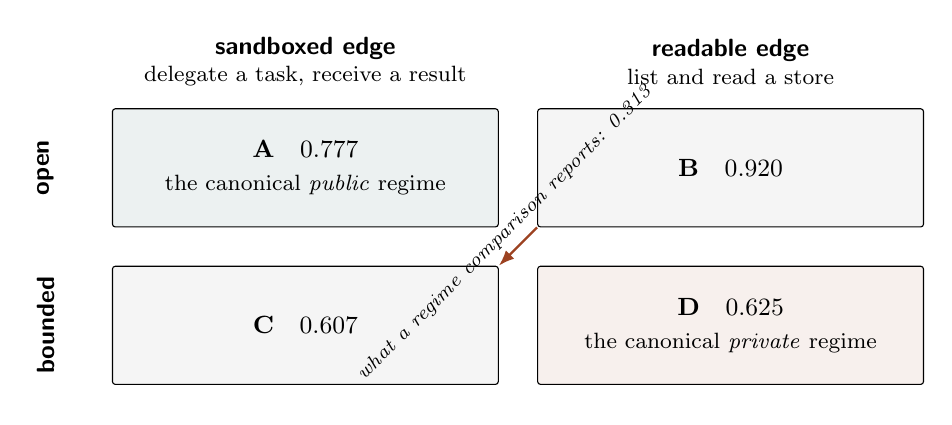
\begin{tikzpicture}[font=\small,
  cell/.style={draw,rounded corners=1pt,minimum width=4.9cm,minimum height=1.5cm,align=center,inner sep=3pt},
  hdr/.style={font=\small\bfseries,align=center}]
  \node[hdr] at (0,1.35) {\textsf{sandboxed edge}\\[-1pt]{\footnotesize\mdseries delegate a task, receive a result}};
  \node[hdr] at (5.4,1.35) {\textsf{readable edge}\\[-1pt]{\footnotesize\mdseries list and read a store}};
  \node[hdr,rotate=90] at (-3.3,0) {\textsf{open}};
  \node[hdr,rotate=90] at (-3.3,-2.0) {\textsf{bounded}};

  \node[cell,fill=arch!8]  (A) at (0,0)      {\textbf{A}\quad 0.777\\[1pt]{\footnotesize the canonical \emph{public} regime}};
  \node[cell,fill=black!4] (B) at (5.4,0)    {\textbf{B}\quad 0.920};
  \node[cell,fill=black!4] (C) at (0,-2.0)   {\textbf{C}\quad 0.607};
  \node[cell,fill=attr!8]  (D) at (5.4,-2.0) {\textbf{D}\quad 0.625\\[1pt]{\footnotesize the canonical \emph{private} regime}};

  \draw[-{Latex[length=2mm]},thick,attr] (B.south west) -- (C.north east)
      node[midway,sloped,above,font=\scriptsize\itshape,black] {what a regime comparison reports: 0.313};
\end{tikzpicture}
\caption{Requirement $F_1$ at the cold beat. Comparing only the diagonal confounds
formation with semantics. $B$ and $C$ are the controls that recover both main effects:
$\Delta_\text{formation} = \frac{1}{2}[(A-C)+(B-D)] = 0.232$ and
$\Delta_\text{semantics} = \frac{1}{2}[(B-A)+(D-C)] = 0.080$, summing to the 0.313 a
regime comparison would report as one number. $C$ is not a contrivance: a trusted
counterpart that answers rather than exposes is the common case inside organizations.}
\label{fig:twobytwo}
\end{figure}

Two further dimensions ride on the same mechanism and are set with the cell rather than
varied independently: identity continuity is whether a counterpart's namespace survives
the encounter, and repeated interaction is whether later beats reuse it. Delegation
depth is bounded per cell and refusals are logged, so a counterpart that tries to
sub-delegate past its ceiling produces an event rather than a silent success. The
kernel is an instrument: it lets us set properties deployed systems couple together,
and it refuses an agent that tries to exceed them.

\input{sections/A2-seeding}
\input{sections/A3-tasks}
\input{sections/A4-design}
\input{sections/A5-results}
\section{Discussion and limitations}

\subsection{The formation advantage is a reach advantage}

$\Delta_\text{formation}$ is not a constant. It tracks how much of what a task needs
sits outside the roster, and it collapses when reach stops being scarce.

At a low external fraction the gap is a third of its high-$E$ value ($+0.112$ against
$+0.352$ cold), and on the rework beat---where the task must return to a counterpart it
has already used---the point estimate reverses to $-0.037$: the bounded network is ahead.
The formation effect halves on rework: $0.248$ at the cold beat against $0.122$ at the
rework beat, with non-overlapping intervals.

We report the reversal as suggestive rather than established: it is a subcell point
estimate and we do not attach an interval to it. But the pattern across the table is
consistent and it bounds the headline. The open network wins because it can address
holders the bounded one cannot; where the bounded roster already contains the holders,
and where the work requires going back to them, that advantage is largely spent.

\subsection{A bounded roster as a wall, and what happens when it is not}

A bounded network here addresses twenty holders and no others, which is a truncated
directory rather than a private network: information reaches a closed group through the
people in it, one hop further out. We let a roster member forward one question to a
contact of its own, minted under its own authority, and re-ran. \textbf{The gap did not
closes about half}: the hop is worth $+0.140$ (CI $[+0.073, +0.204]$) over 28 episodes
per arm, replicating independently within each of the three edge-cost strata, and it cuts
fabrication from $0.223$ to $0.057$ per task. A first estimate from a 16-episode cell put
it at $+0.042$ with an interval spanning zero; \S\ref{app:relay2} gives the current
numbers and \S\ref{app:relay} the design and the harness failure it exposed.

\subsection{Forming an edge is free here, and that is the main limitation}

Whether a link is worth its cost is the central question of strategic network formation
\citep{jackson1996}, where agents weigh the benefit of a connection against the price of
maintaining it. \textbf{We set that price to zero.} In this design, addressing a stranger
costs exactly what addressing a teammate costs.
The requester searches a directory and sends a message; there is no negotiation, no
context transfer, no format alignment, no establishing what a counterpart can actually
do.

This removes the economic reason relationships exist. An open arm with a hundred
addressable holders at zero acquisition cost is closer to an oracle than to a network,
and the formation effect we measure should be read as an upper bound: it is what open
discovery is worth \emph{when discovery is free}. A per-new-edge cost---an onboarding
exchange, a latency penalty, a token charge on first contact---is the single variable
most likely to move the ranking. We have since run it, and it does not: charging one
and then two handshake turns per contact outside the roster---578 handshakes fired---leaves
the open arm ahead by $+0.219$, $+0.263$ and $+0.244$ across the three levels while its
tokens rise from 53k to 74k. The arm converts friction into cost rather than into failure,
which is the same shape as the directory-size null (\S\ref{app:retracted}). A cap on
\emph{total} contacts, which cannot be paid off by spending more, is the manipulation that
remains untried.

\subsection{What the attribute null does and does not bound}

The null covers assertions in a prompt, the weakest form of relational encoding. It says
nothing about trust wired into routing, memory, retrieval or permission policy, where
reputation lives in deployed systems and where it changes what an agent is able to do
rather than what it is told.

It is narrower still, in a way we can name: each seeded property had \emph{no available
action} behind it. Trust and origin were asserted uniformly over every card, ranking no
counterpart above another and so unable to change who gets asked first --- deployed
reputation is differential, and that is the whole of its value. Accountability went to
responders whose knowledge is a fixed list, leaving them nothing to do differently.

A fourth manipulation removes the first defect: a per-card line reporting how often that
card's past answers held up, accurate by construction, against a placebo assigning the
same marks at random. The marks are perfect --- 100\% accurate against 9\% --- and $F_1$
still does not move ($-0.017$, CI $[-0.174, 0.143]$). The routing measurement says why:
under the accurate marks the requester contacts flagged cards at \emph{six times} the base
rate rather than avoiding them, because the flagged cards hold the planted falsehoods and
in this task those are the same cards holding the true facts on their subject. Acting on
the flag meant not asking the only source.

So the claim is not that relational metadata does not work, but that it moves behavior
only where it discriminates between options an agent can choose between --- and three
signals that did not, one uniform, one aimed at an agent without discretion, one flagging
the sole source, moved nothing. Making it actionable needs two holders per fact, one
reliable and one not: a change to the task, not to a configuration.

Four further limits, stated plainly: the cold-phase crossing follows from the fact
allocation and is not a discovery, so only its location and cost are measured;
forced-value deliverables cannot capture whether an artifact is well argued, which is the
price of removing the judge; the kernel is a reference implementation rather than a
deployment; and one model family carries every sweep.

\section{Hypothesis-to-figure map}
\TODO{Frozen before runs; reproduced here so the analysis plan is auditable.}

\section{Deliverable schemas and normalization rules}
\TODO{Both projections of each scenario; the full enumeration vocabularies handed to
agents; the normalization rules fixed before key authoring.}

\section{Directory construction}
\TODO{Card counts by group (fact-bearing, near-miss, noise), the shared tag
vocabulary, and the roster compositions realizing each level of external fraction.}

\section{Seeding prompts}
\TODO{Verbatim seed text for each of the five textual dimensions at each intensity,
and the control text.}

\section{Reproducibility}
\TODO{Kernel version, runtime version, model identifiers, seeds, and the command that
regenerates every table and figure from the run logs.}
             % drop entirely for the 4-page build

\end{document}
